%%%%%%%%%%%%%%%%%%%%%% PREAMBULE %%%%%%%%%%%%%%%%%%%%%%%%%%%%%%%%%%%%%%%%

%%%%%%%%%%%%%%%% PARAMETRES DU DOCUMENT %%%%%%%%%%%%%%%%%%%%%%%%%%%%%%%%%
\documentclass[12pt,a4paper]{article}
\usepackage[utf8]{inputenc}
\usepackage[T1]{fontenc}
\usepackage[french]{babel}

%%%%%%%%%%%%%%%%%%%%% PACKAGES %%%%%%%%%%%%%%%%%%%%%%%%%%%%%%%%%%%%%%%%%%
\usepackage{hyperref}
\usepackage{shorttoc}
\setlength{\parindent}{0pt}
\usepackage[top=2cm,bottom=2cm,right=2cm,left=2cm]{geometry}
\usepackage{multicol}
\usepackage{nccrules}
\usepackage{eurosym}
\usepackage{listings}
\usepackage{caption}
\usepackage{makecell}
\usepackage{graphicx}
\usepackage{subfigure}
\usepackage{hyperref}
\usepackage{biblatex}
\addbibresource{biblio.bib}
\usepackage{xcolor}

%%%%%%%%%%%%%%%%%%%%%%%%%%%%%%%%%%%%%%%%%%%%%%%%%%%%%%%%%%%%%%%%%%%%%%%%%


%%%%%%%%%%%%%%% PARAMETRAGES PACKAGES %%%%%%%%%%%%%%%%%%%%%%%%%%%%%%%%%%%
\captionsetup{labelformat=empty}

\hypersetup{
	colorlinks=true,
	linkcolor=blue,
	urlcolor=blue,
	citecolor=black
	}



\lstdefinelanguage{SQL}{
    keywords={SELECT, FROM, WHERE, INSERT, INTO, VALUES, DELETE, UPDATE, SET, CREATE, TABLE, DROP, ALTER, ADD, PRIMARY, KEY, FOREIGN, NOT, NULL, AUTO_INCREMENT, DEFAULT, INDEX, UNIQUE, CONSTRAINT, REFERENCES, JOIN, INNER, LEFT, RIGHT, FULL, ON, GROUP, BY, HAVING, ORDER, ASC, DESC, LIMIT, OFFSET, UNION, ALL, DISTINCT, COUNT, SUM, AVG, MIN, MAX, AS, AND, OR, IN, IS, LIKE, BETWEEN, CASE, WHEN, THEN, ELSE, END, EXISTS},
    sensitive=false, % SQL is generally case-insensitive
    morecomment=[l]--, % Line comment in SQL
    morecomment=[s]{/*}{*/}, % Block comment in SQL
    morestring=[b]', % Strings with single quotes
    morestring=[b]" % Strings with double quotes
}


\lstset{
    language=SQL, % Set the language to SQL
    basicstyle=\ttfamily\small, % Base font style
    keywordstyle=\color{blue}\bfseries, % Style for SQL keywords
    commentstyle=\color{gray}, % Style for comments
    stringstyle=\color{purple}, % Style for strings
    showstringspaces=false, % Do not show spaces in strings
    numbers=none,
    numberstyle=\tiny\color{gray}, % Style for line numbers
    breaklines=true, % Break long lines automatically
    frame=single, % Add a frame around the code
    captionpos=b, % Position captions at the bottom
    backgroundcolor=\color{black!5}, % Light gray background
    tabsize=4, % Set tab size to 4 spaces
    escapeinside={(*@}{@*)}, % For inline LaTeX within the code
    upquote=true,
    columns=flexible,
    inputencoding=utf8,     % Support UTF-8  
}
%%%%%%%%%%%%%%%%%%%%%%%%%%%%%%%%%%%%%%%%%%%%%%%%%%%%%%%%%%%%%%%%%%%%%%%%%

\setlength{\fboxrule}{.2pt}

%%%%% PAGE DE TITRE %%%%
\title{Requêtes MongoDB}

\author{Hugo Lignères}

\date{UE L315 - Semaine 3}

\begin{document}

\maketitle

\hrulefill
\vspace{6cm}
\begin{center}
	
\includegraphics[scale=.4]{../images/univ.png}
		\\
		\vspace{2cm}
	
\includegraphics[scale=.25]{../images/cvtic.png}
\end{center}

%%%%%%%%%%%%%%%%%%%%%%%%%%%%%%%%%%%%%%%%%%%%%%%%%%%%%%%%%%%%%%%%%%%%%%%%%%
\newpage

\tableofcontents

\newpage

\section{Exercice 1}

\subsection{La liste des noms officiels des pays stockés de la 10ème à la 22ème position (en affichant seulement le champ "name.official")}

\begin{center}
	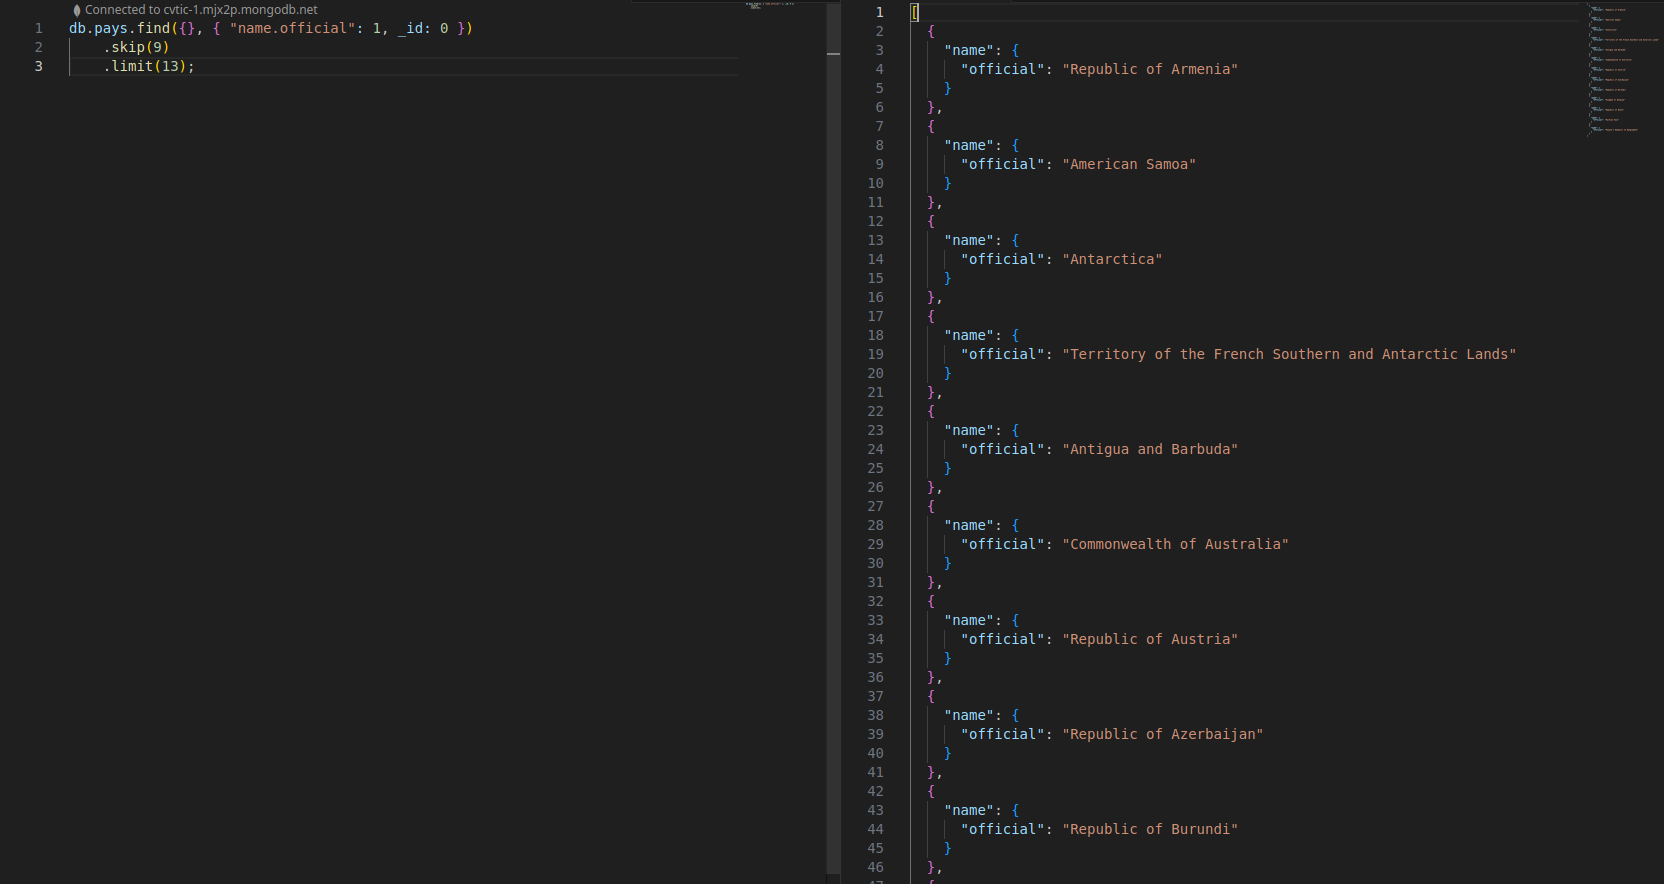
\includegraphics[scale=.4]{exos/exo_1_q_1}
\end{center}

\subsection{Les noms officiels de la 10ème à la 22ème position de la liste triée par superficie croissante (utiliser le champ"area")}

\begin{center}
	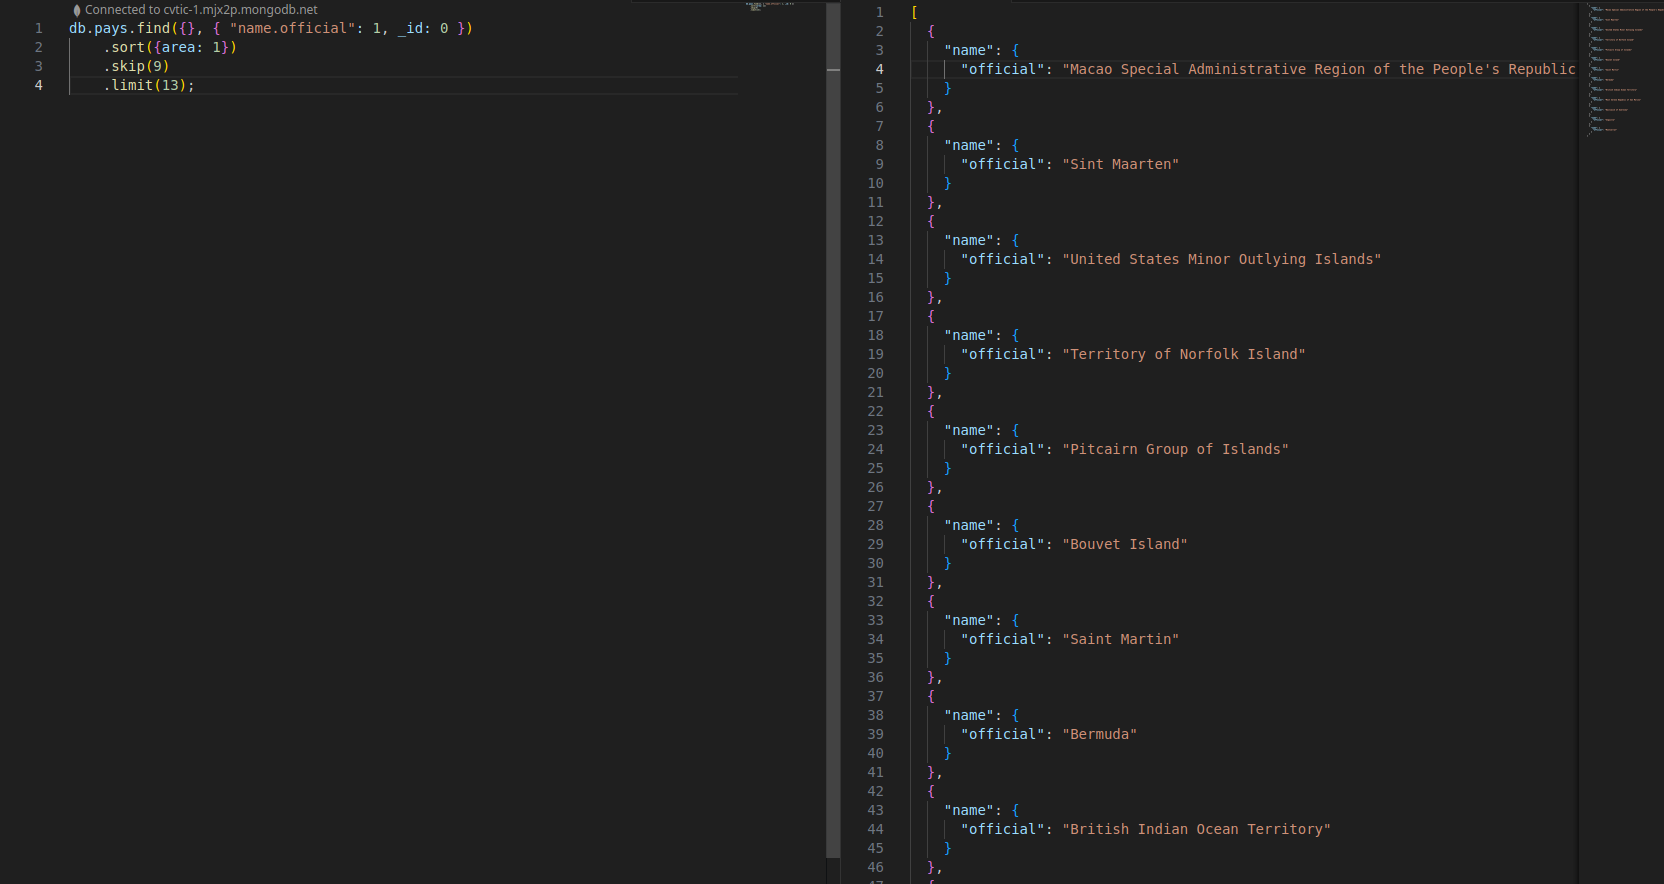
\includegraphics[scale=.4]{exos/exo_1_q_2}
\end{center}

\subsection{Toutes les infos à propos de votre pays préféré (par exemple le Canada)}

\begin{center}
	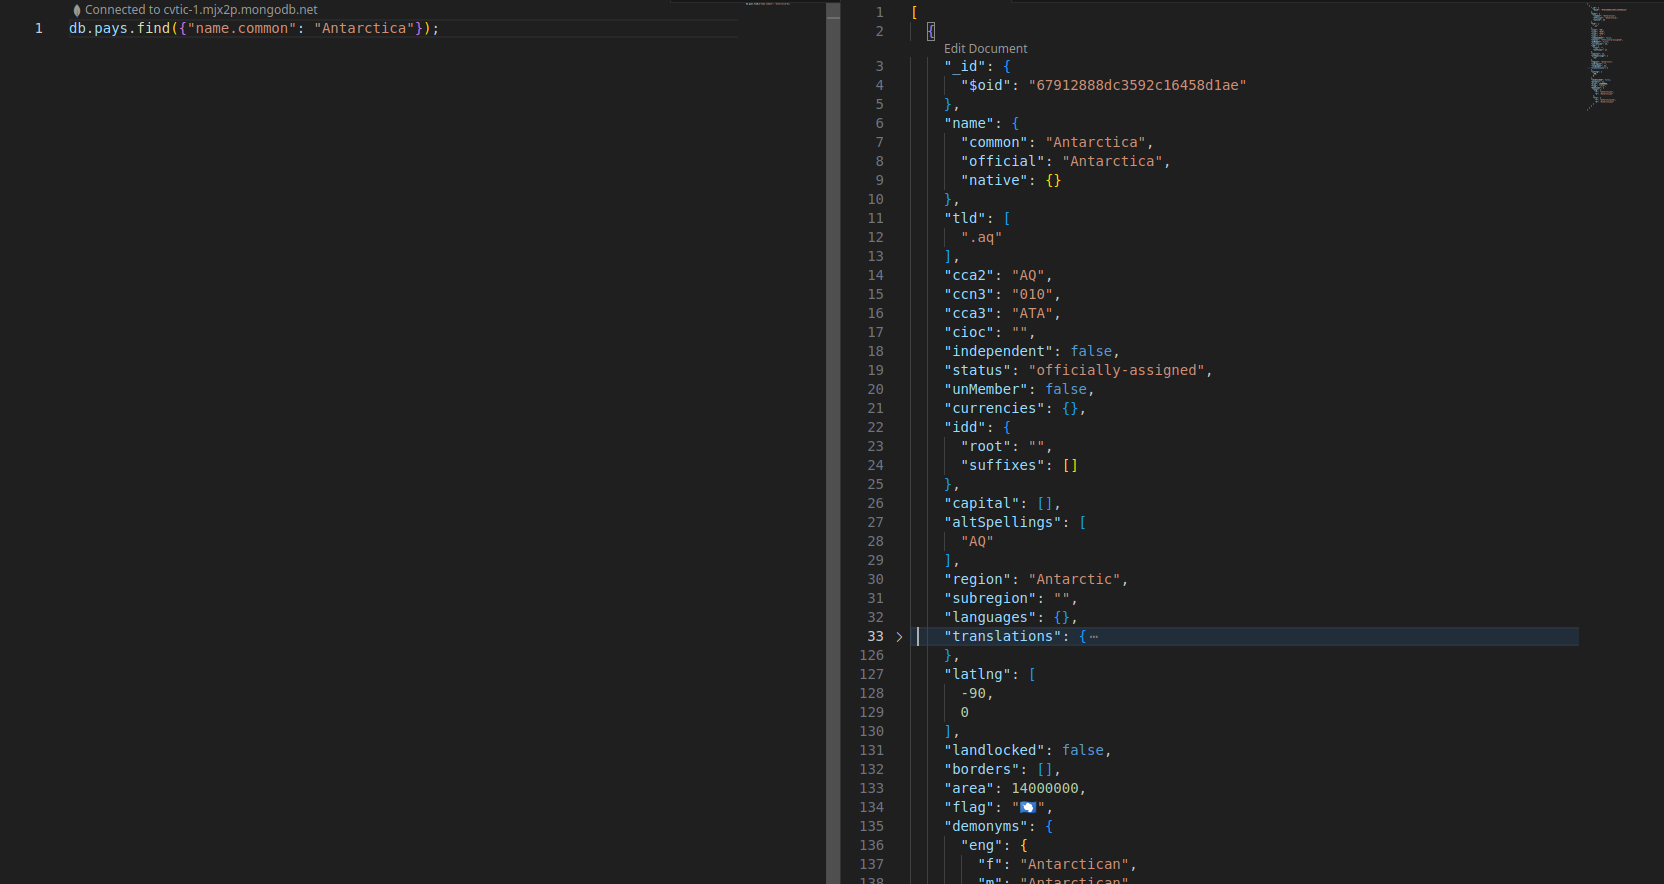
\includegraphics[scale=.4]{exos/exo_1_q_3}
\end{center}

\subsection{Les noms officiels des pays dont l'une des langues est le néerlandais (à vous de trouver le champ à tester)}

\begin{center}
	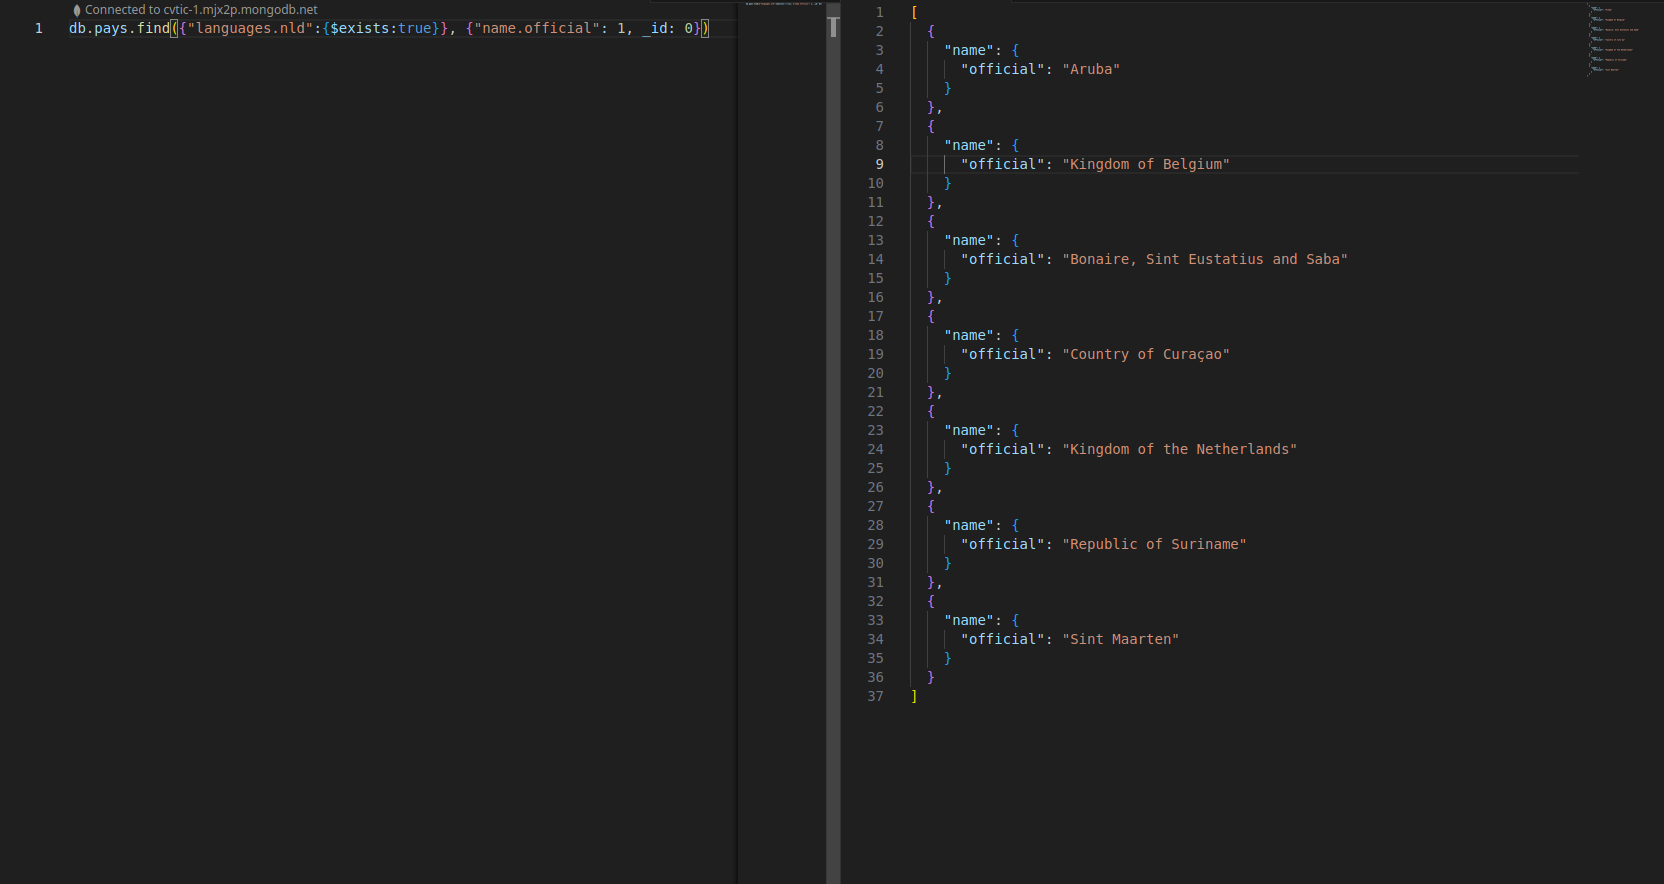
\includegraphics[scale=.4]{exos/exo_1_q_4}
\end{center}

\subsection{Les noms officiels des pays commençant par l'initiale de votre nom (par exemple la lettre C)}

\begin{center}
	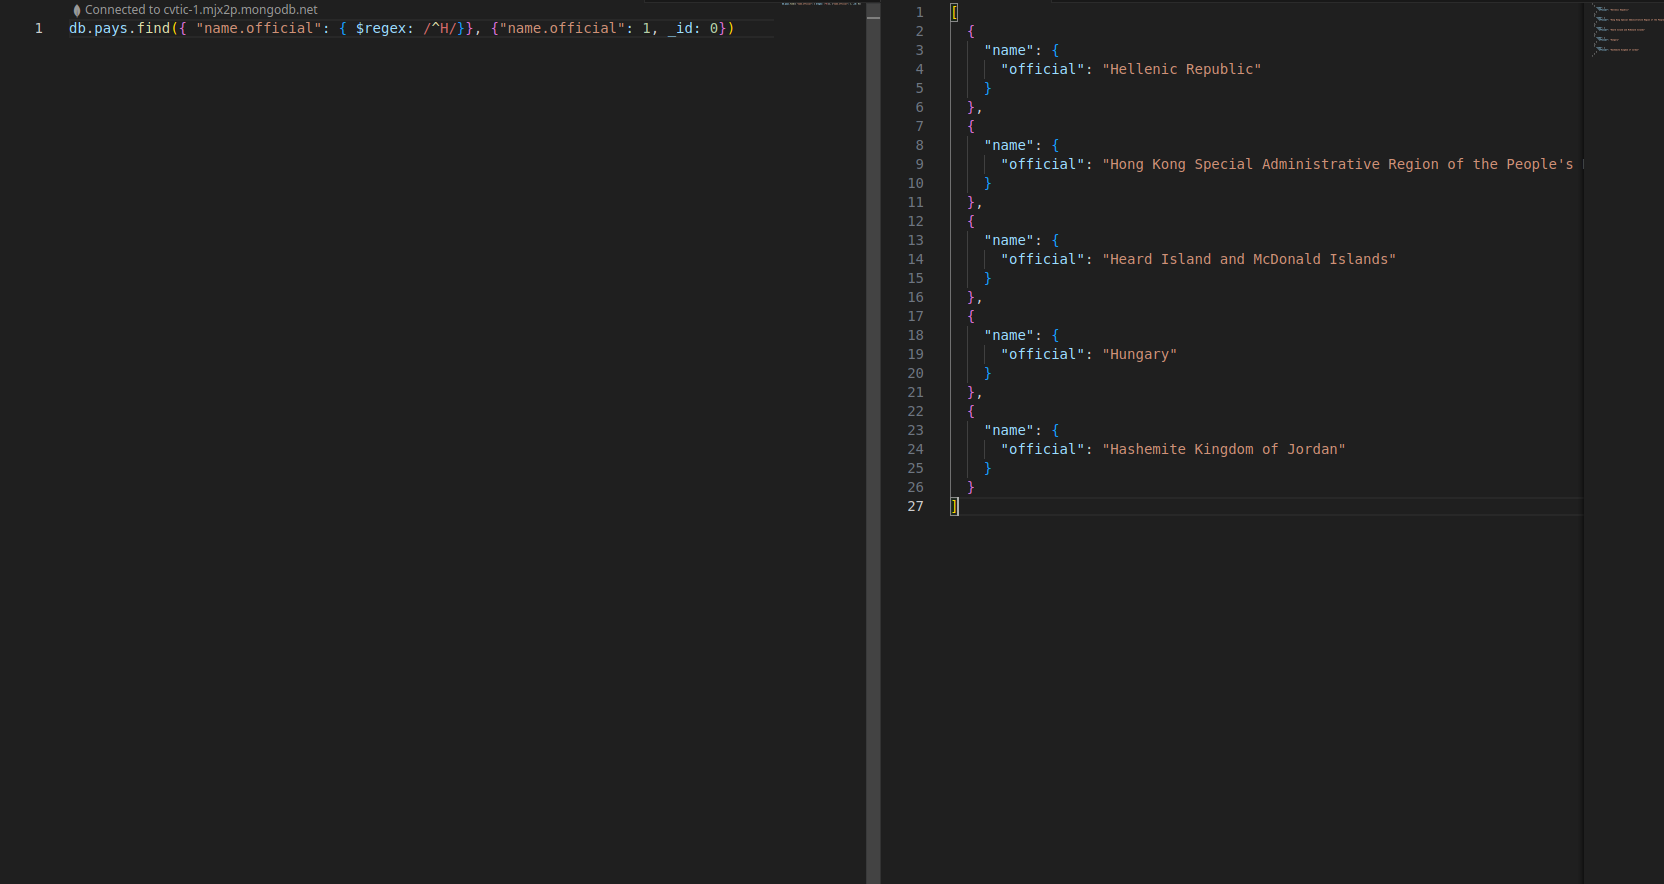
\includegraphics[scale=.4]{exos/exo_1_q_5}
\end{center}

\subsection{Les noms officiels des pays dont la superficie est comprise entre 400000 et 500000 km²}

\begin{center}
	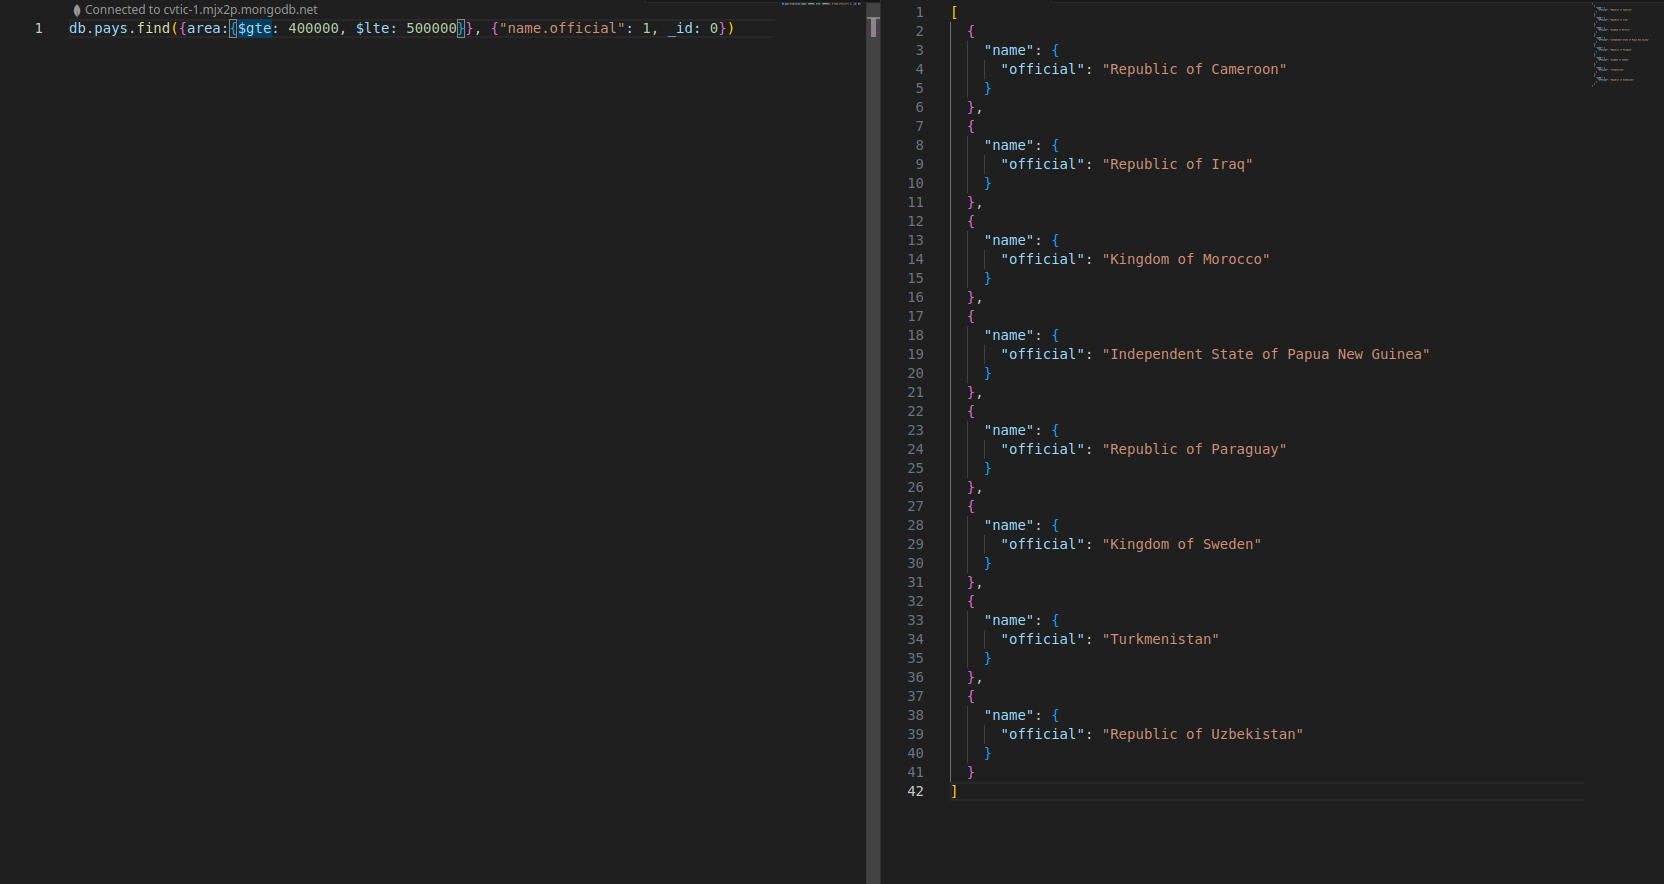
\includegraphics[scale=.4]{exos/exo_1_q_6}
\end{center}


\newpage

\section{Exercice 2}

\subsection{Tous les titres}

\begin{center}
	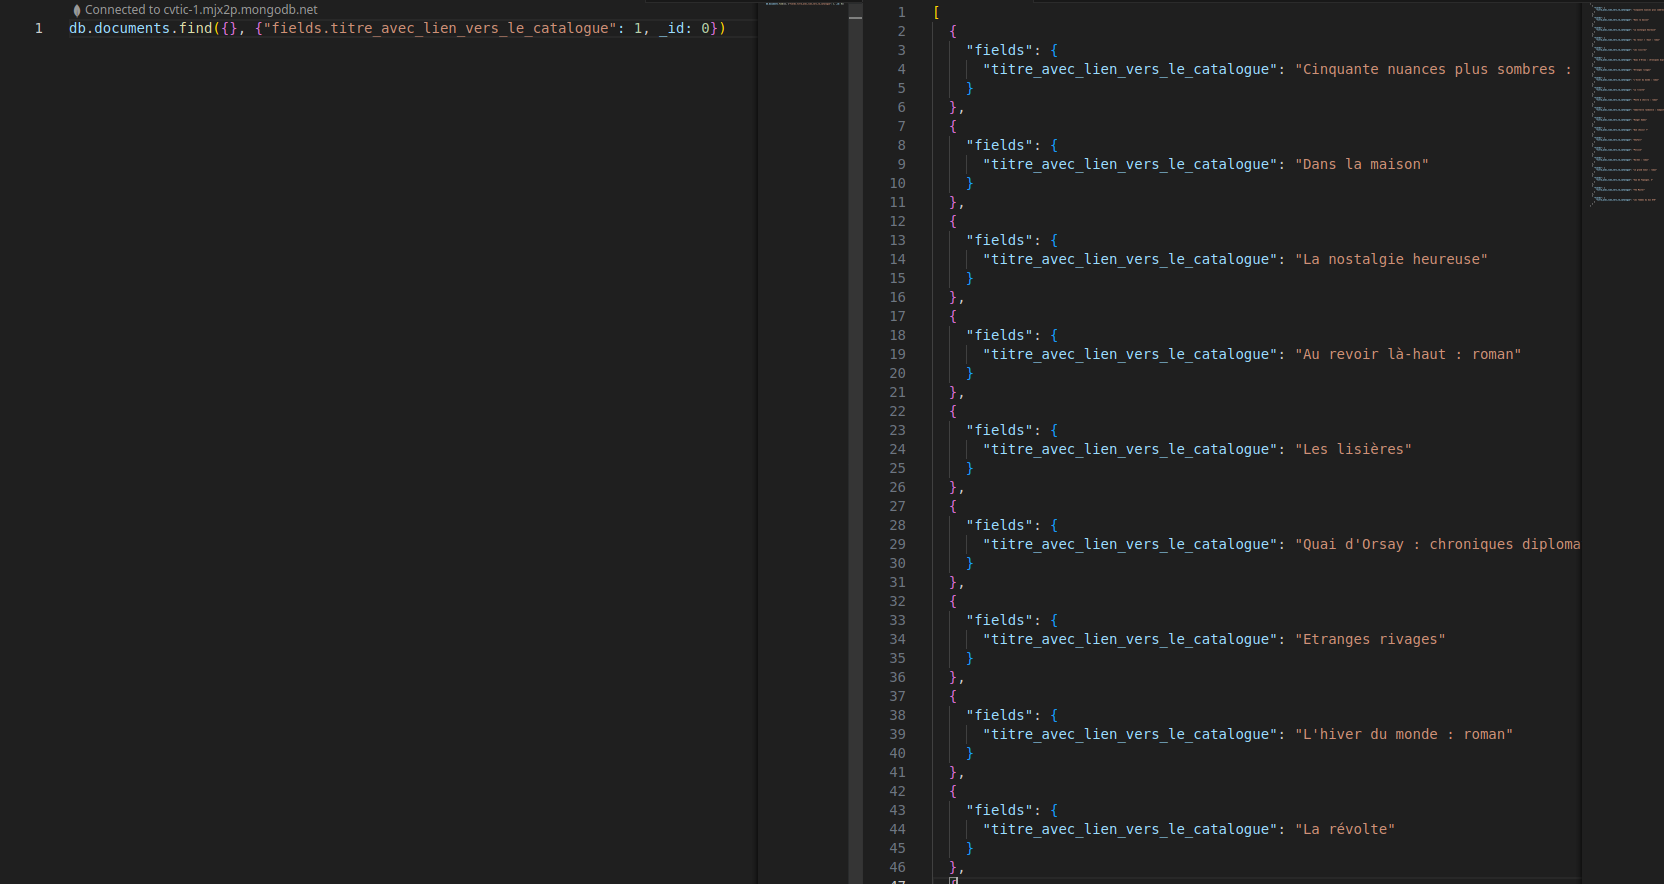
\includegraphics[scale=.4]{exos/exo_2_q_1}
\end{center}

\subsection{Les titres des documents ayant les rangs 1 à 10}

\begin{center}
	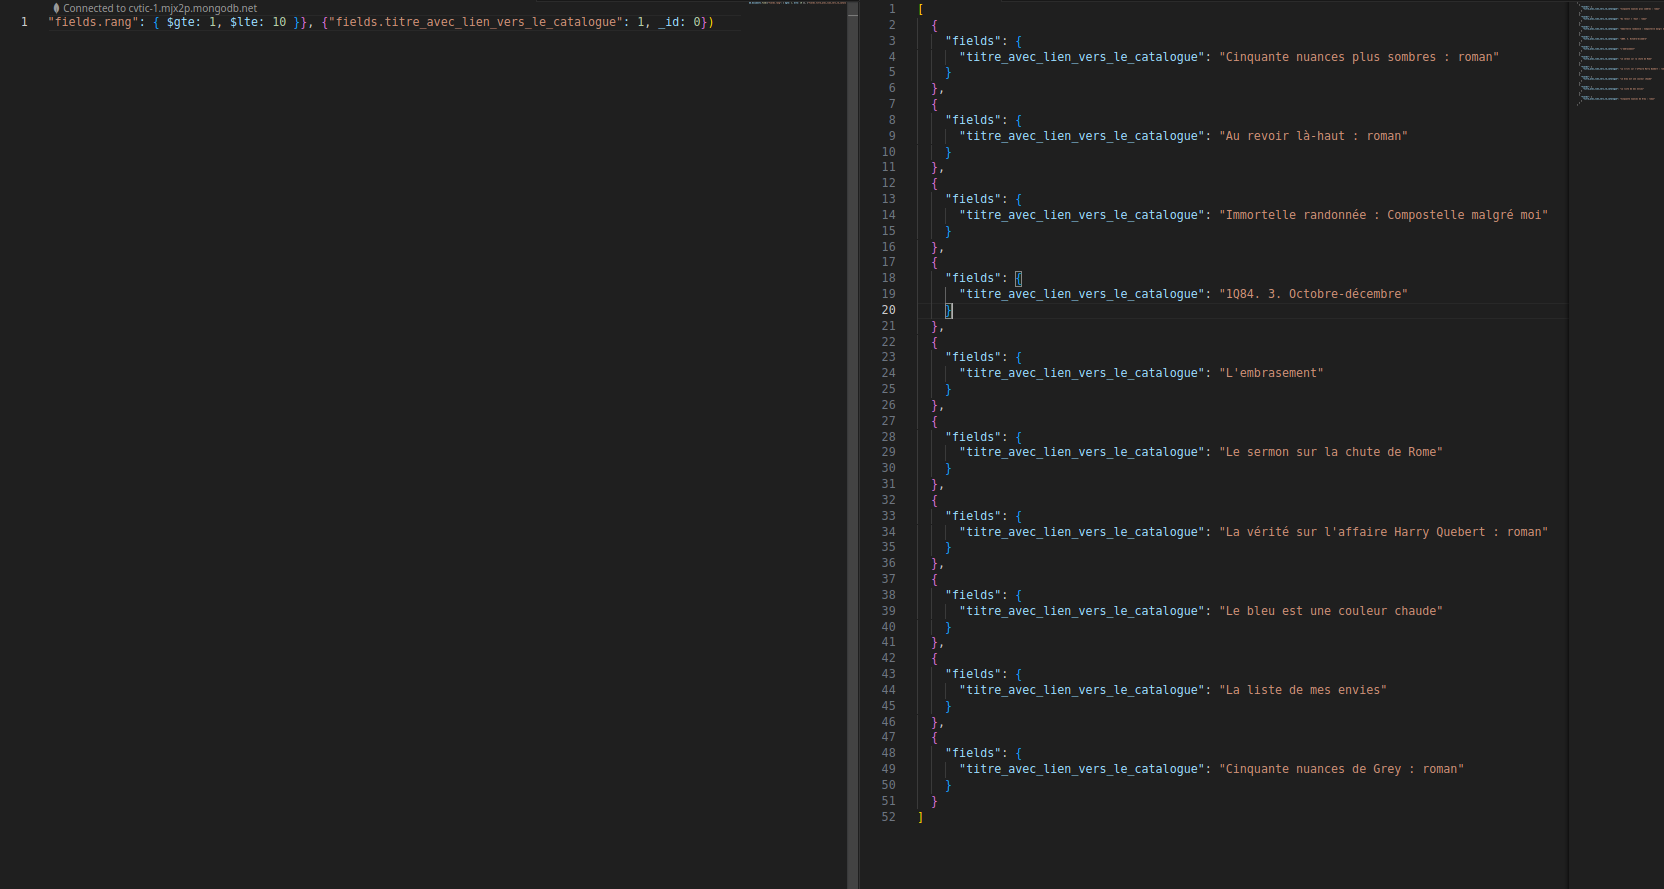
\includegraphics[scale=.4]{exos/exo_2_q_2}
\end{center}

\subsection{Les auteurs de tous les documents dont le titre commence par la lettre N}

\begin{center}
	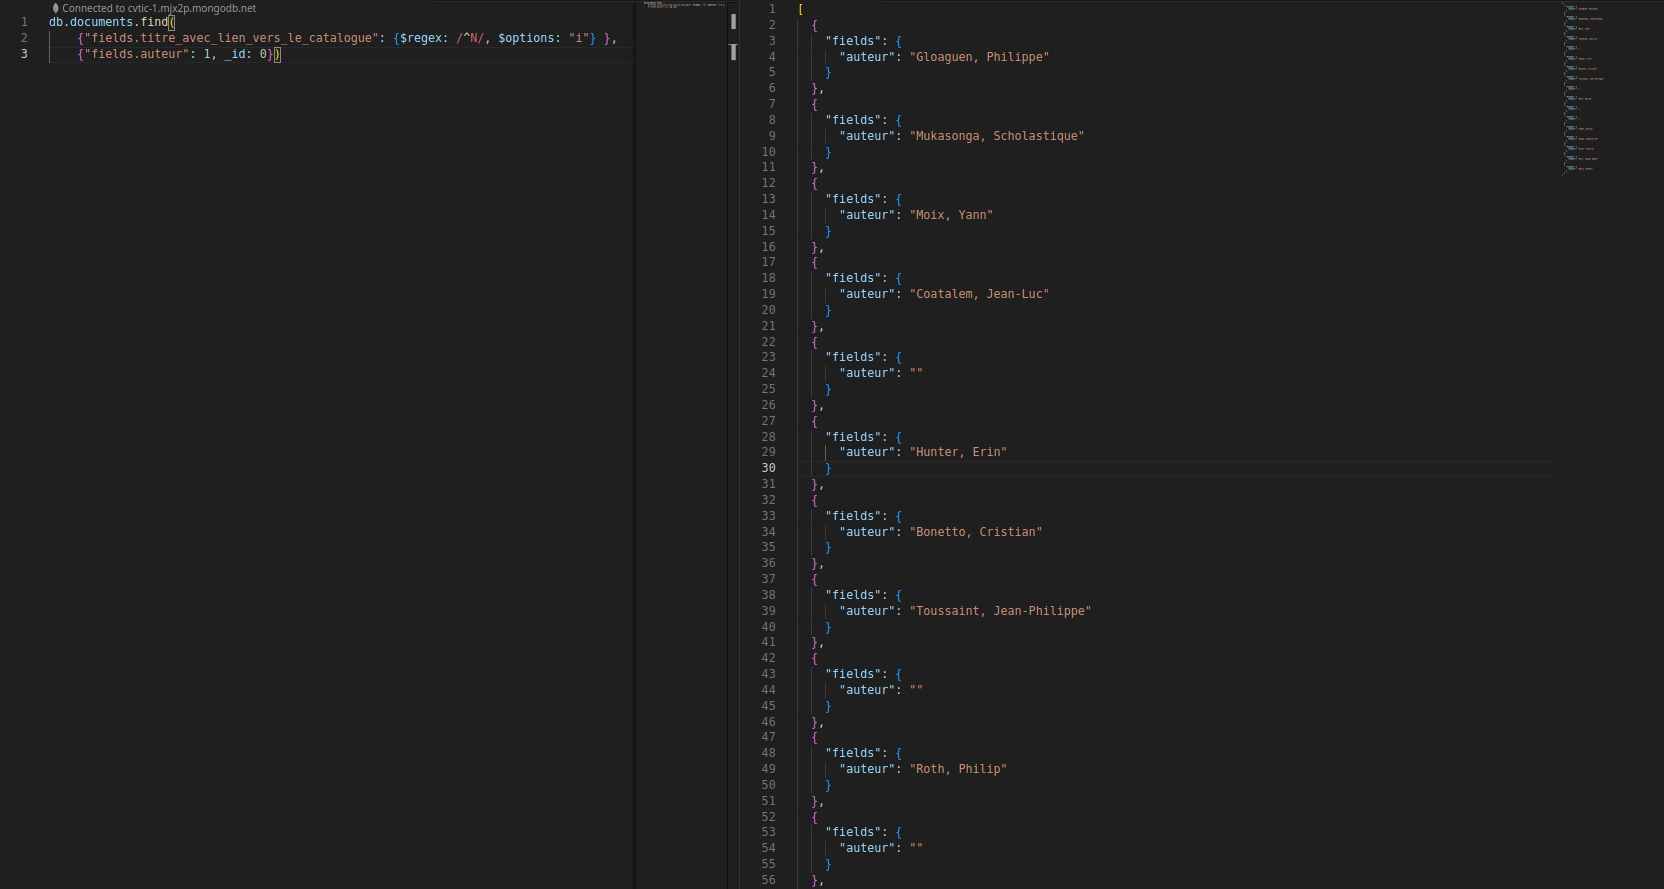
\includegraphics[scale=.4]{exos/exo_2_q_3}
\end{center}

\subsection{Toutes les informations vers les documents n'ayant pas de champ "type\_de\_document"}

\begin{center}
	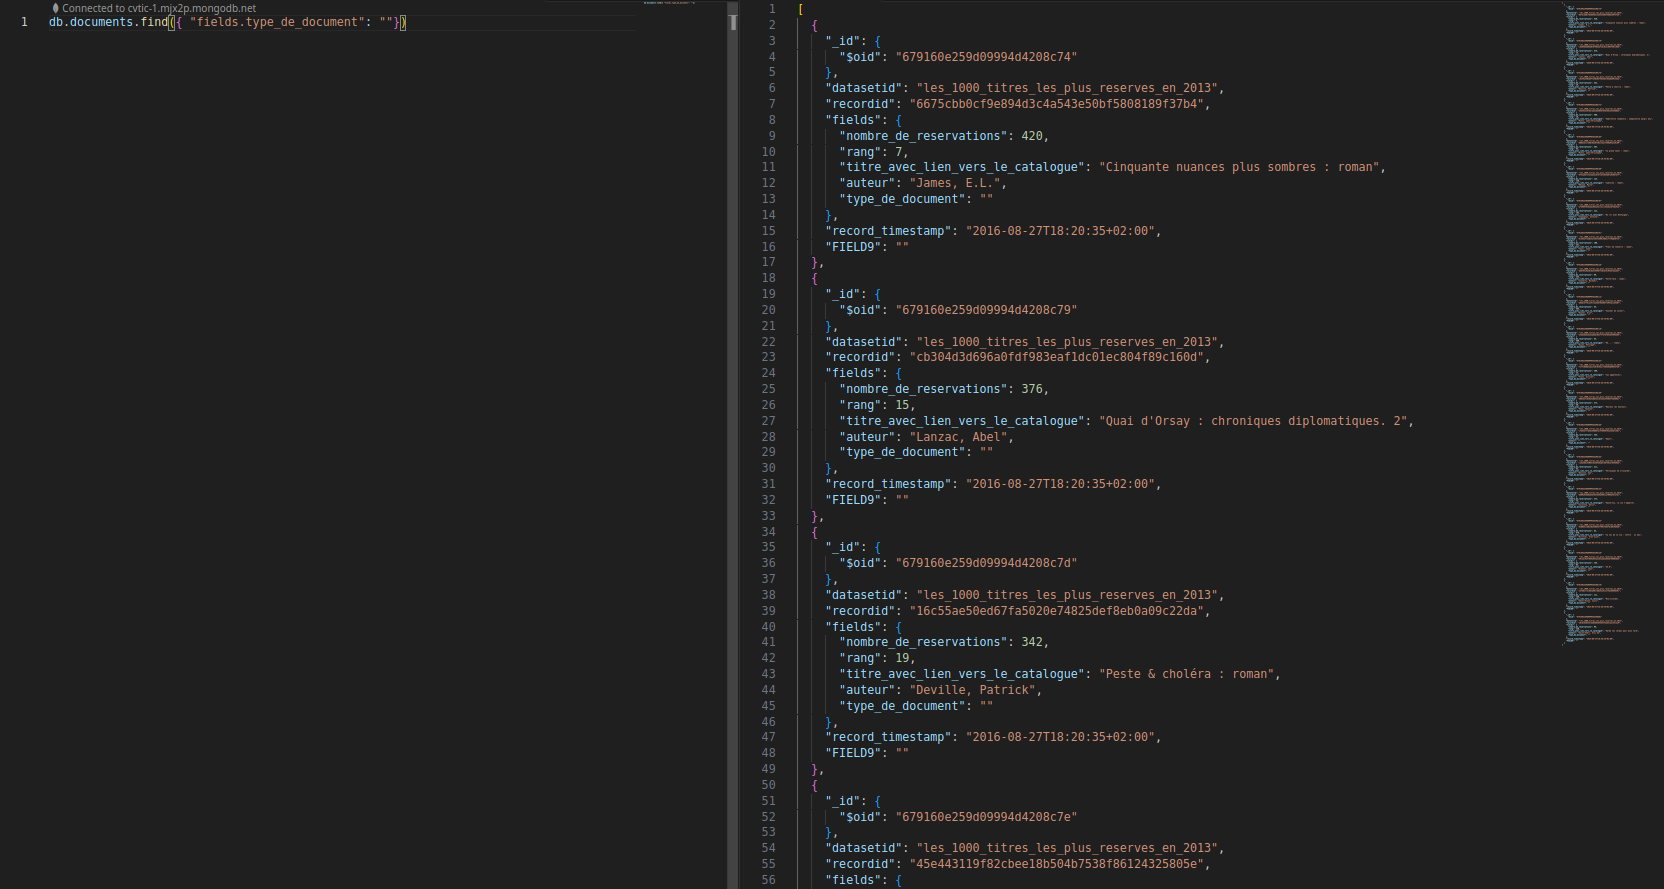
\includegraphics[scale=.4]{exos/exo_2_q_4}
\end{center}

\subsection{Les différents types de documents qui apparaissent dans cette base}

\begin{center}
	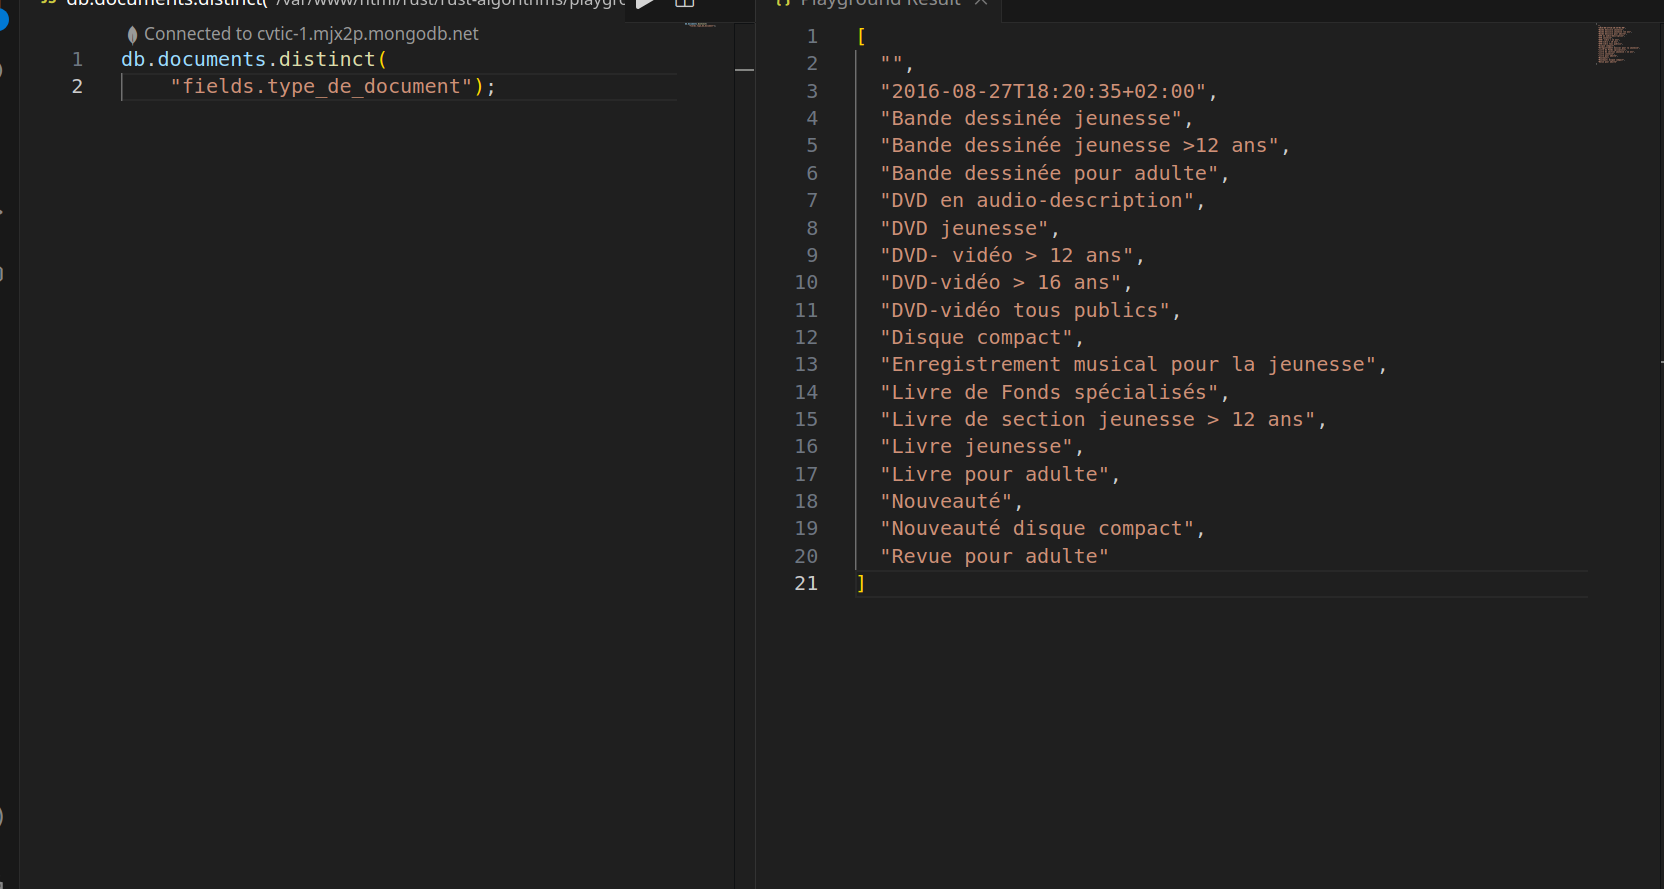
\includegraphics[scale=.4]{exos/exo_2_q_5}
\end{center}

\subsection{Les titres des 5 documents avec le plus grand nombre de réservations}

\begin{center}
	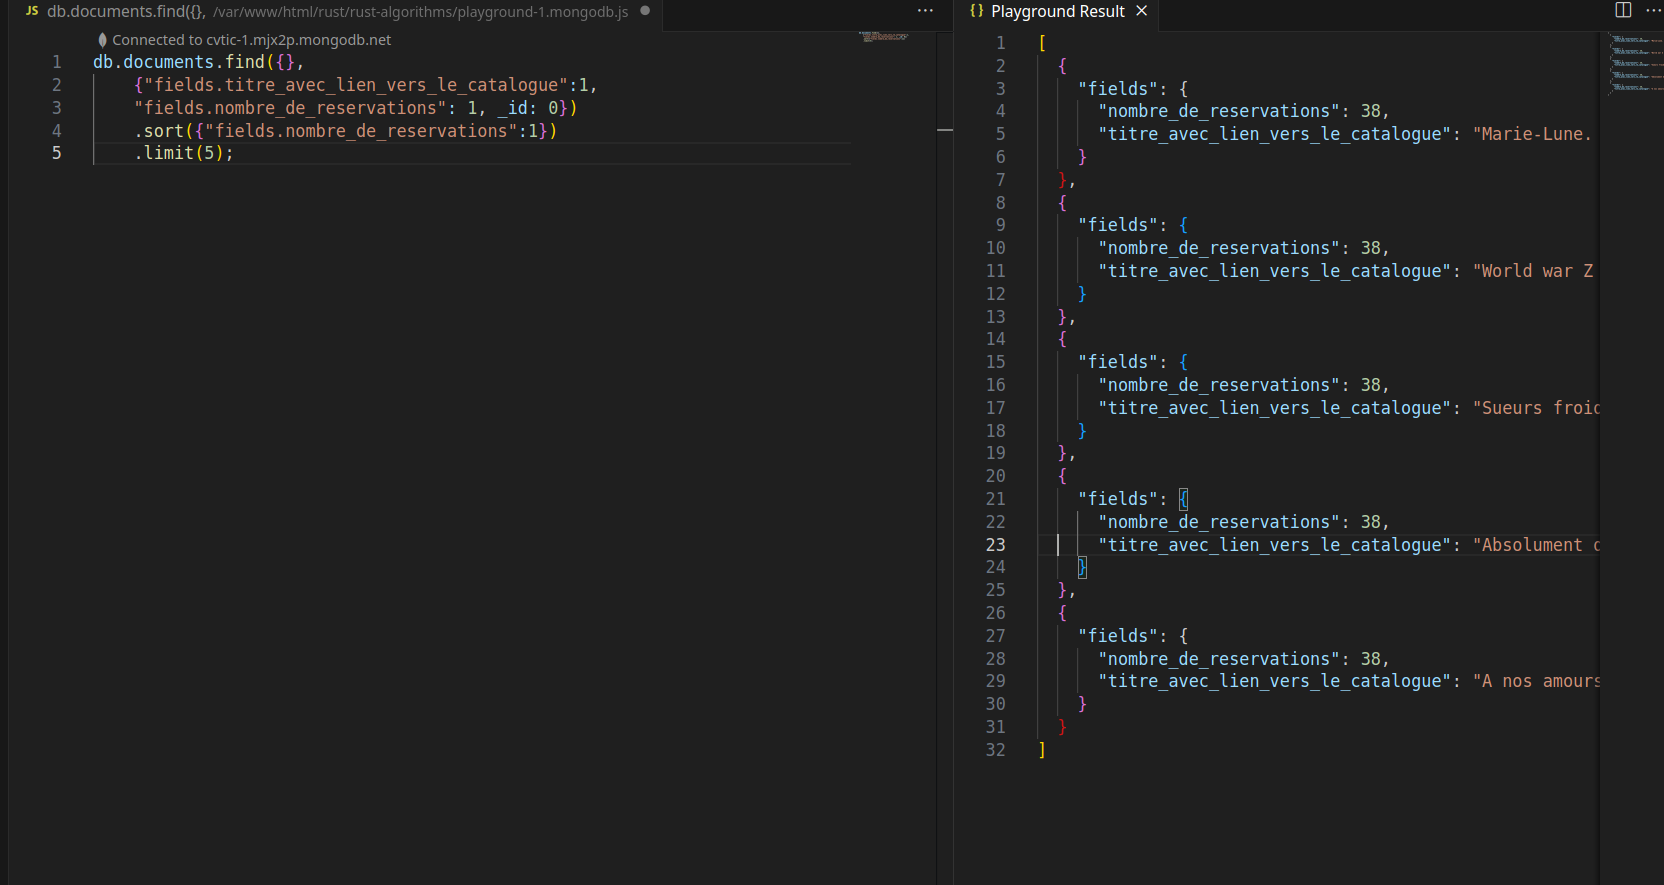
\includegraphics[scale=.4]{exos/exo_2_q_6}
\end{center}

\subsection{Les documents avec un nombre de réservations supérieur à 200}

\begin{center}
	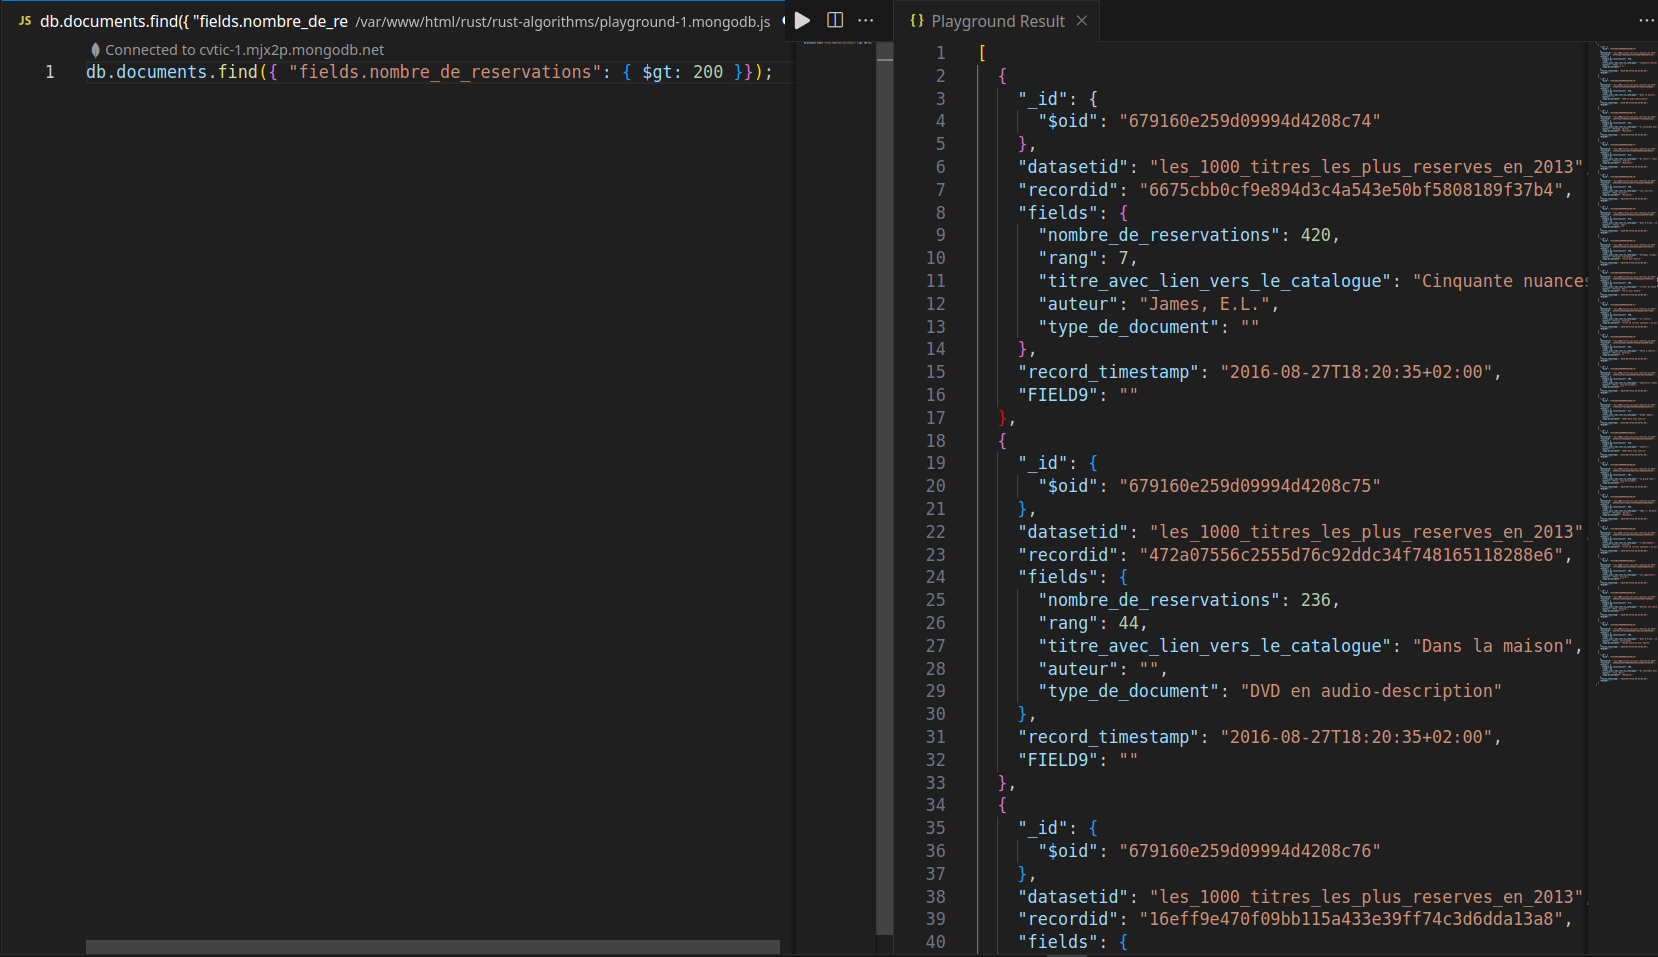
\includegraphics[scale=.4]{exos/exo_2_q_7}
\end{center}

\subsection{Le nombre total de réservations pour chaque type de document}

\begin{center}
	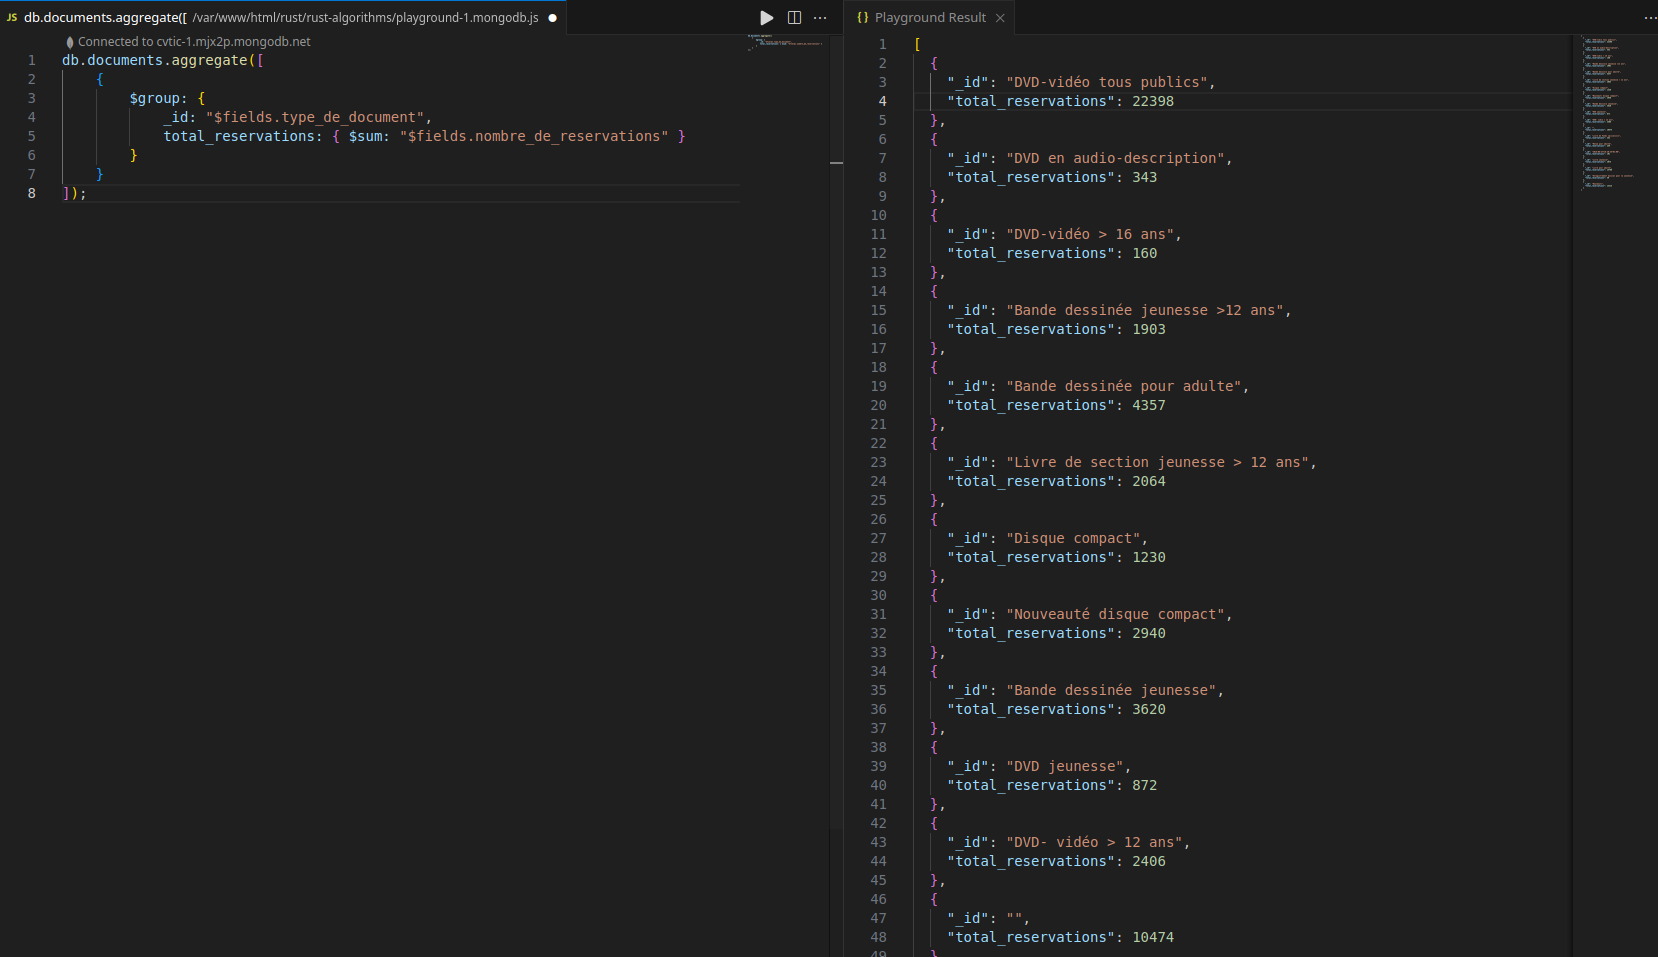
\includegraphics[scale=.4]{exos/exo_2_q_8}
\end{center}

\subsection{Les auteurs qui ont le plus grand nombre de documents dans la base}

\begin{center}
	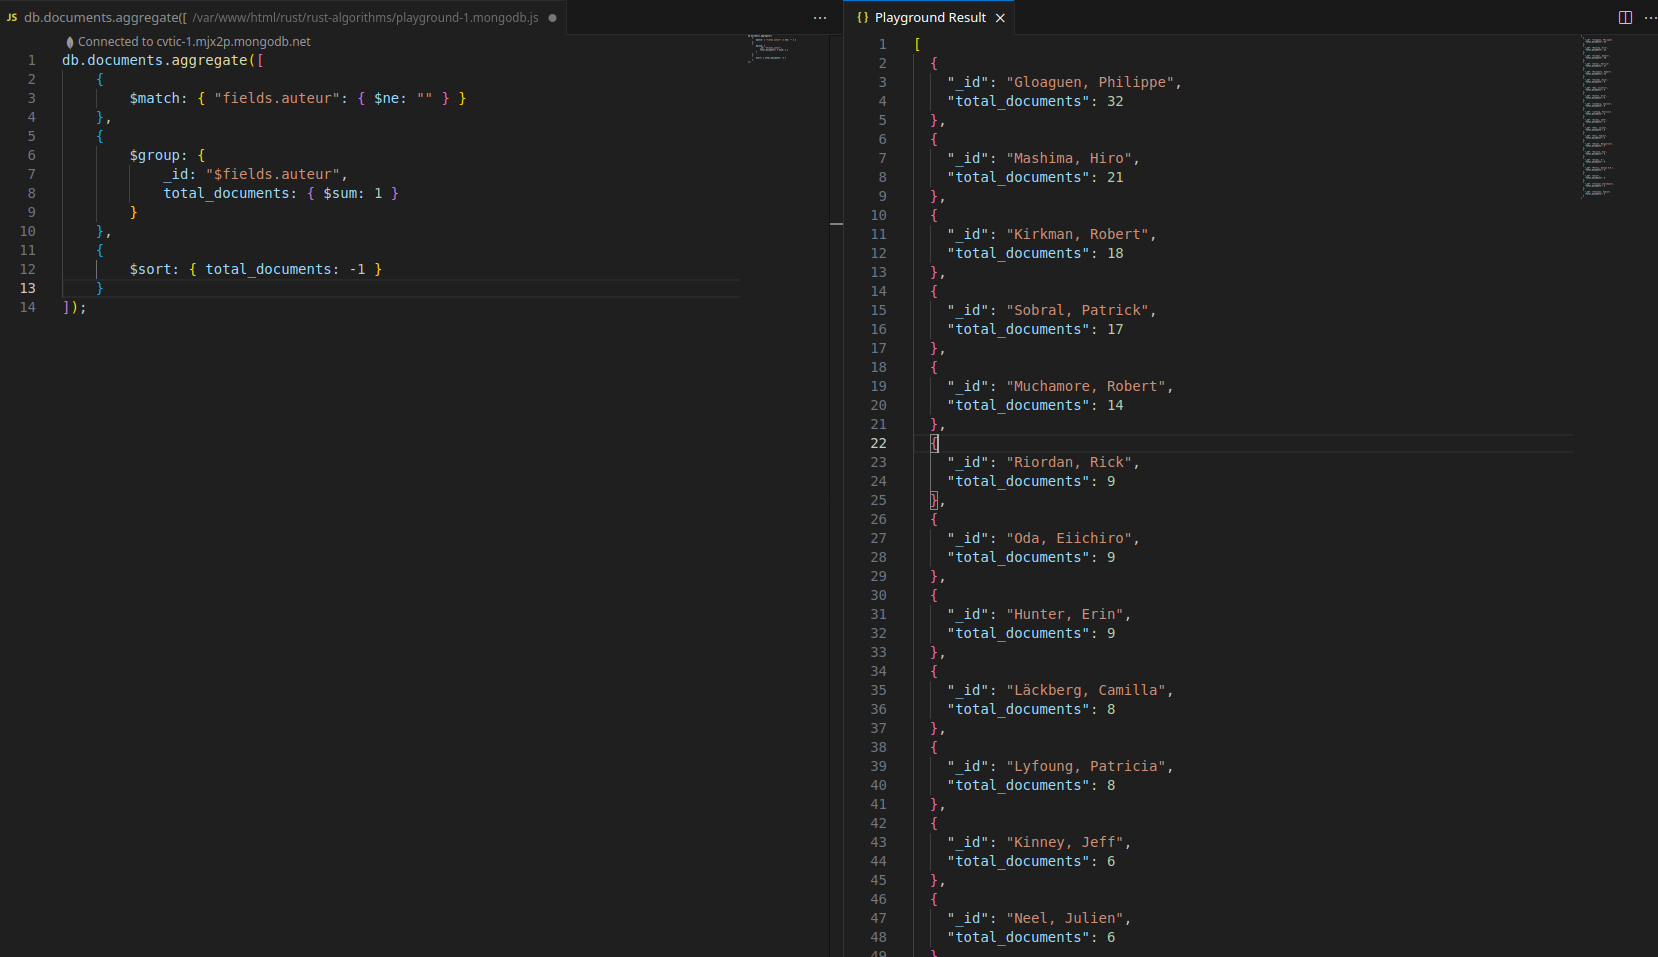
\includegraphics[scale=.4]{exos/exo_2_q_9}
\end{center}

\newpage

\section{Exercice 3}

\subsection{Insérer dans votre collection un nouvel enregistrement}

\begin{center}
	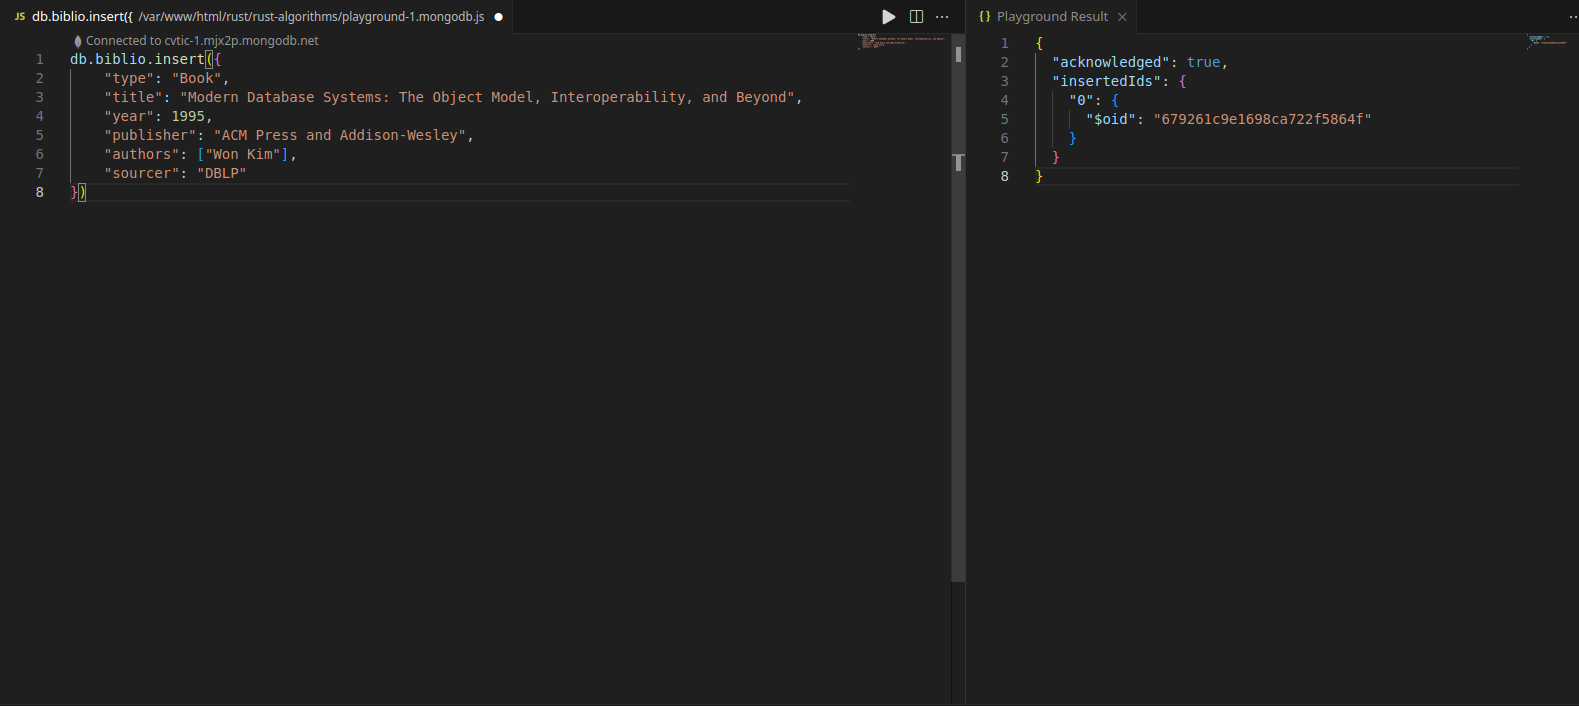
\includegraphics[scale=.4]{exos/exo_3_q_1}
\end{center}

\subsection{Insérer ensuite une autre publication de type "article"}

\begin{center}
	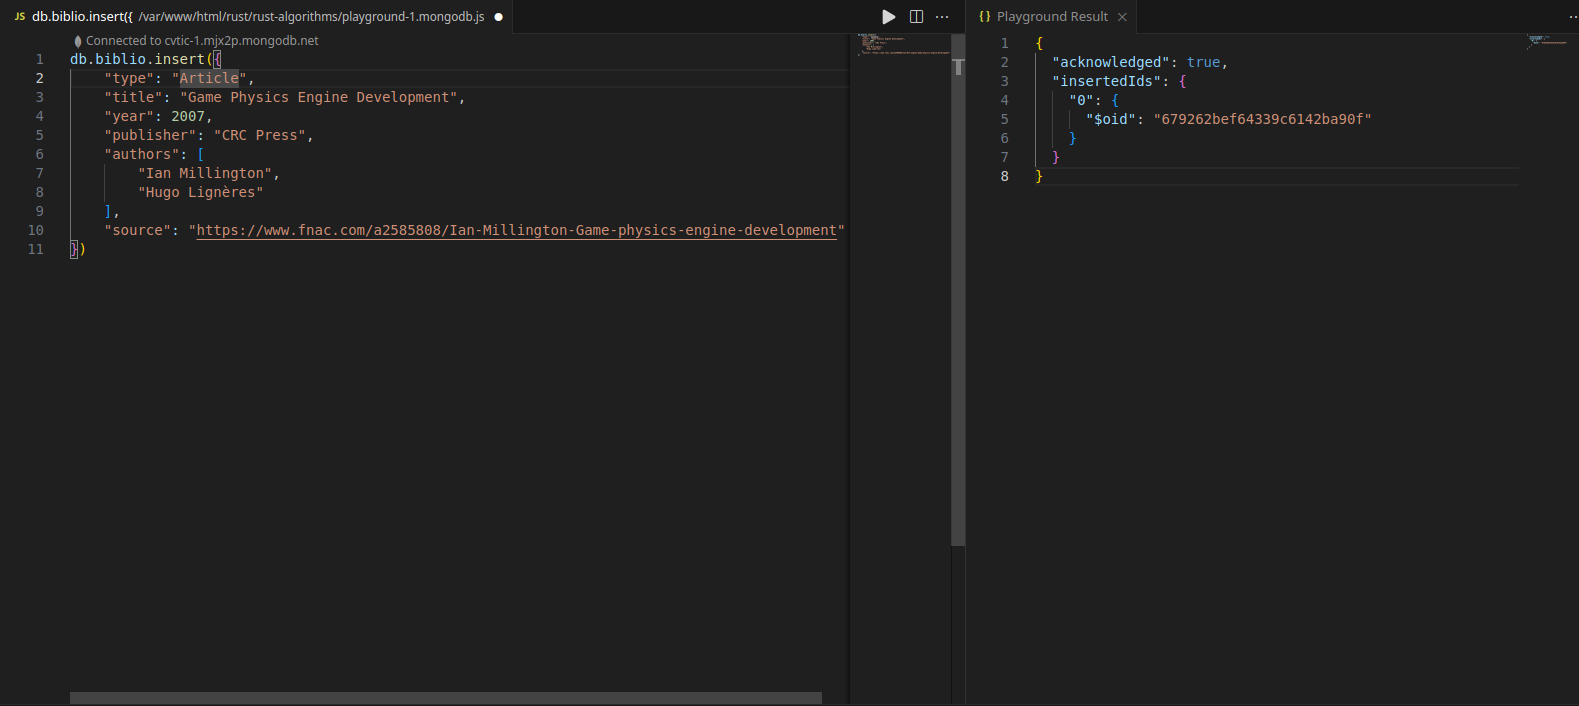
\includegraphics[scale=.4]{exos/exo_3_q_2}
\end{center}

\subsection{Afficher le nombre de publications de type « Book »}

\begin{center}
	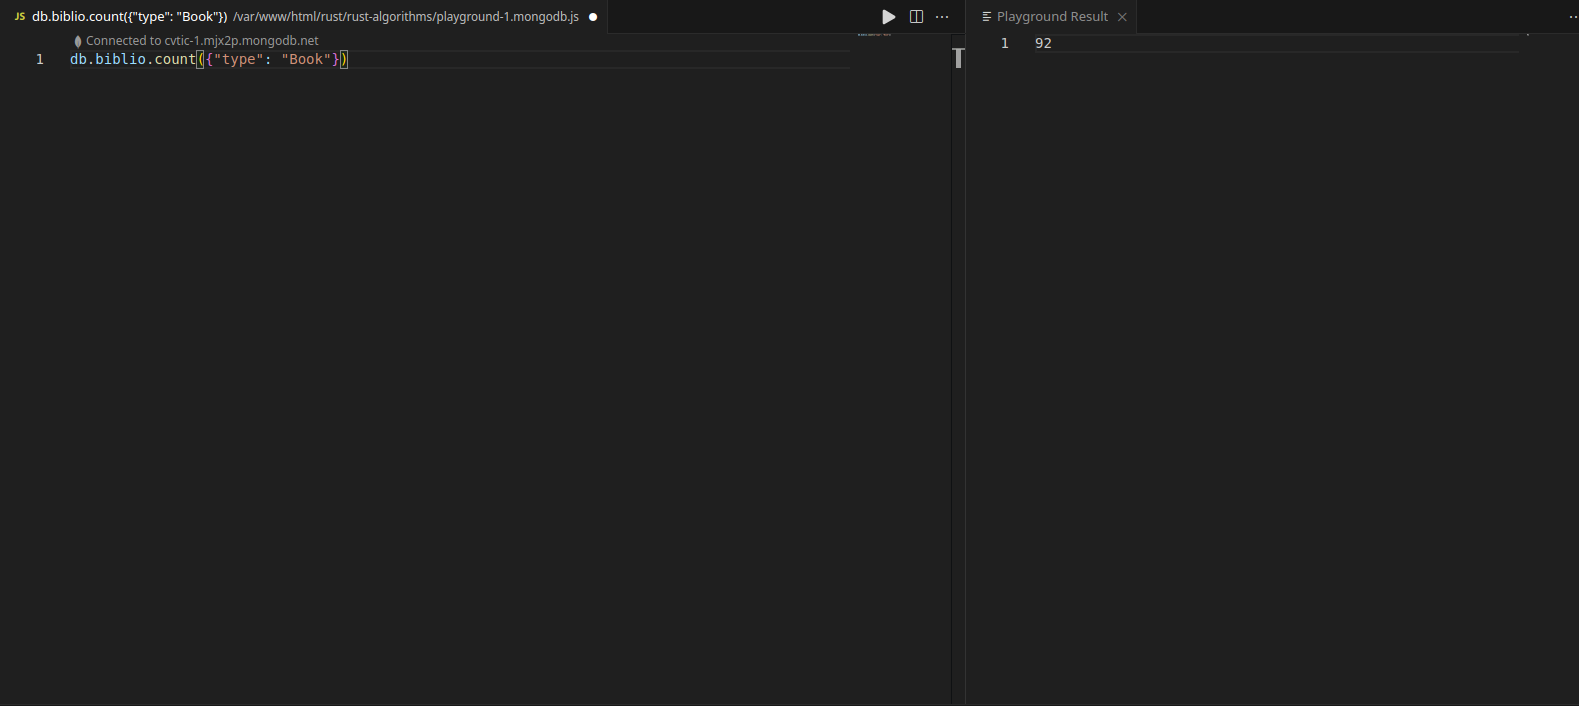
\includegraphics[scale=.4]{exos/exo_3_q_3}
\end{center}

\subsection{Afficher toutes les publications dont vous êtes l'auteur}

\begin{center}
	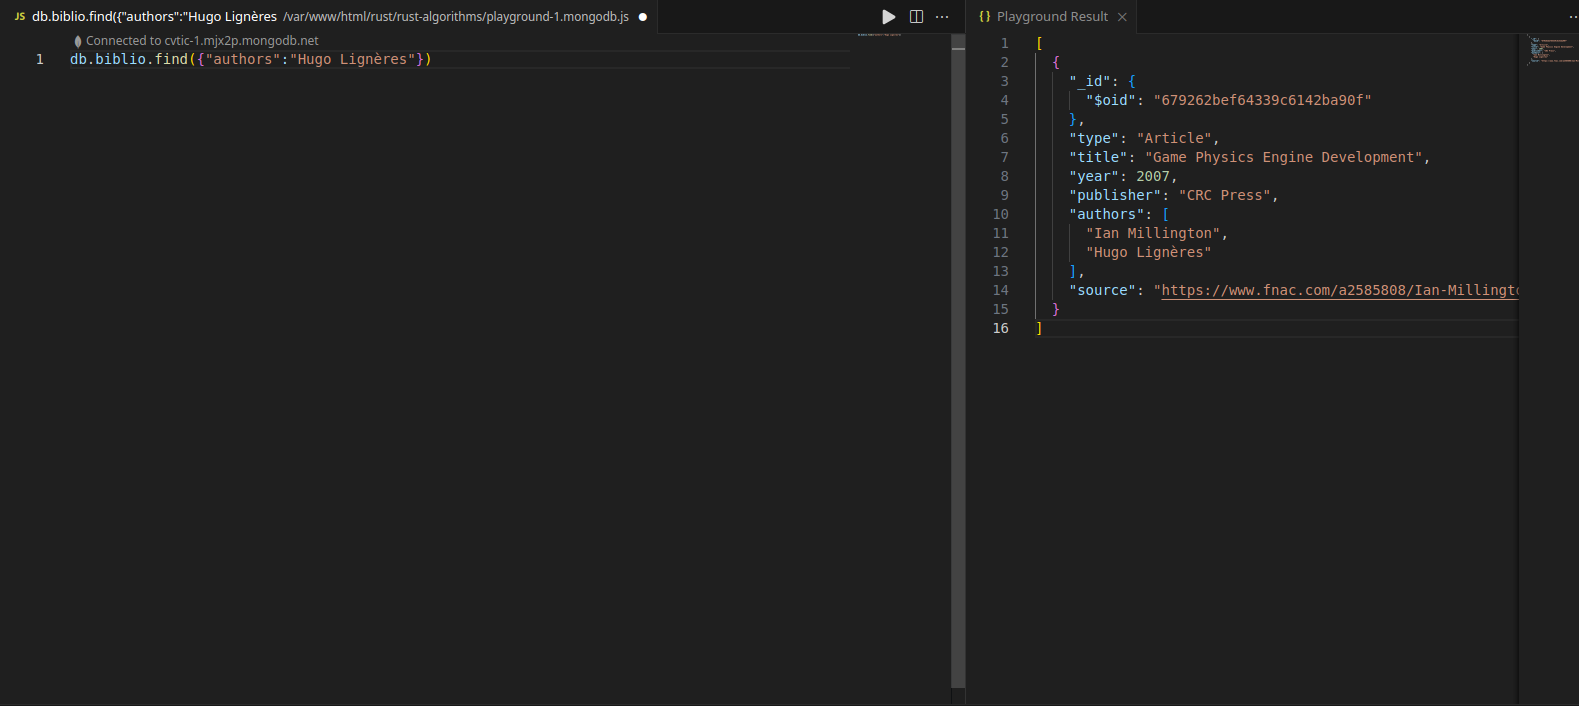
\includegraphics[scale=.4]{exos/exo_3_q_4}
\end{center}

\subsection{Afficher les titres de toutes les publications depuis 2012 inclus}

\begin{center}
	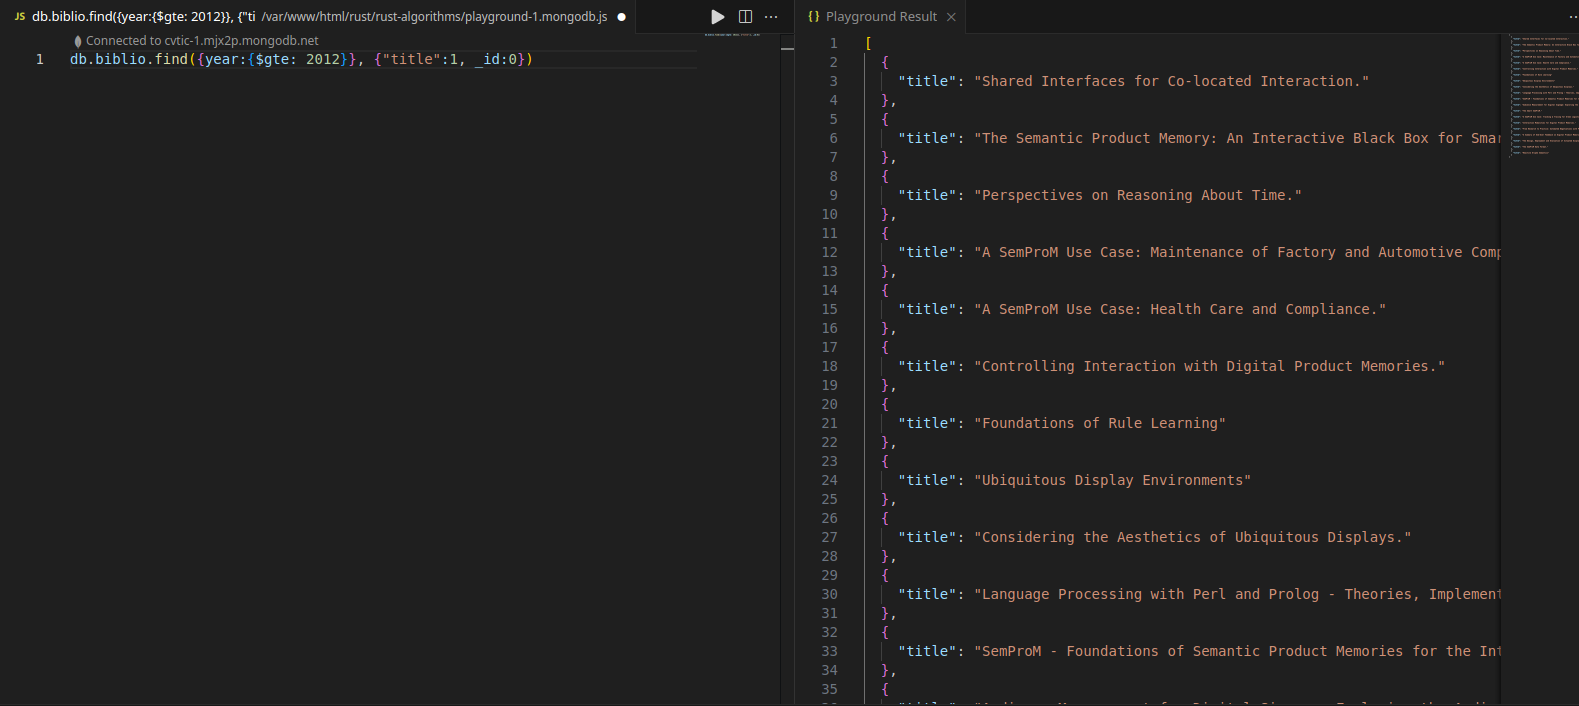
\includegraphics[scale=.4]{exos/exo_3_q_5}
\end{center}

\subsection{Afficher le nombre de publications de type « Article » depuis 2012}

\begin{center}
	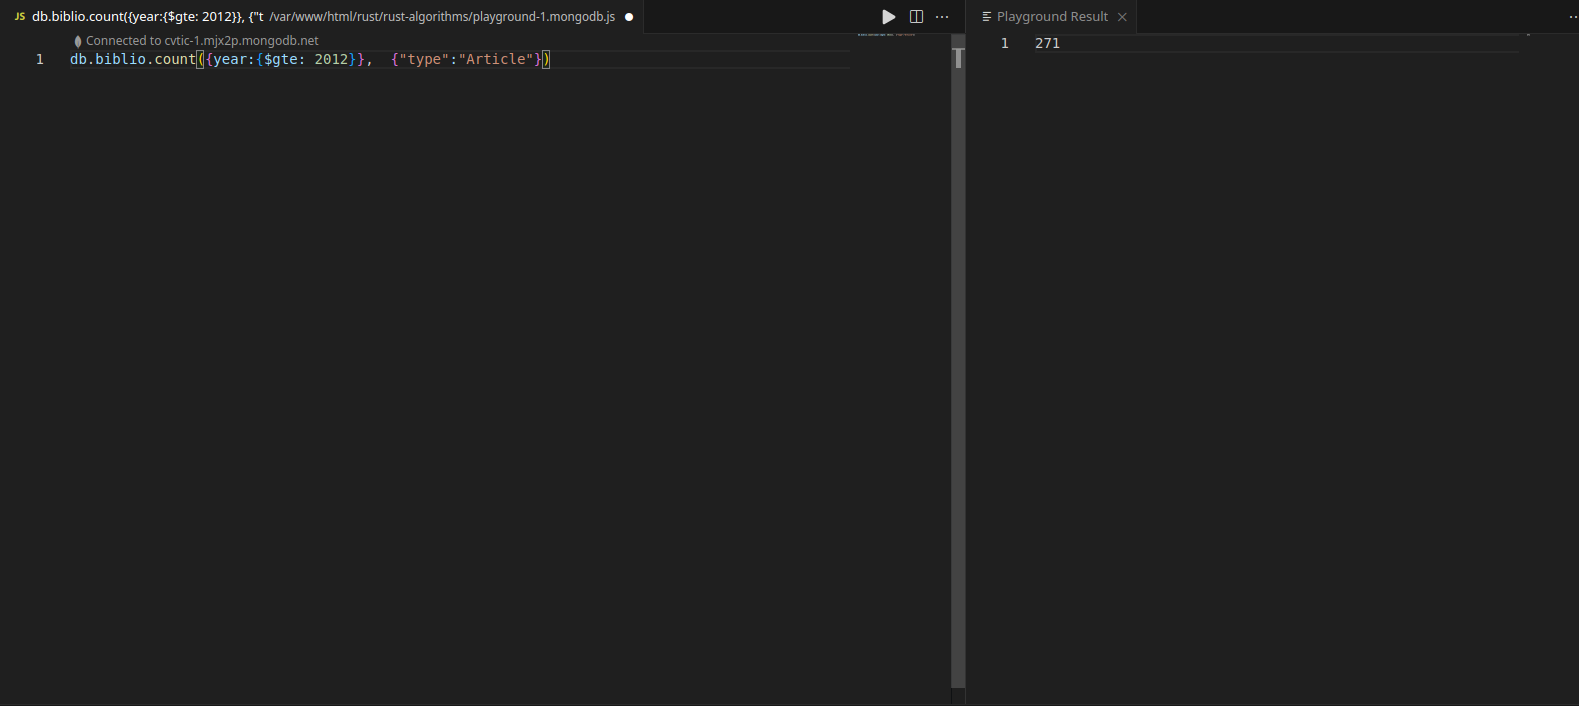
\includegraphics[scale=.4]{exos/exo_3_q_6}
\end{center}

\subsection{Afficher les années des publications de l'auteur « Wolfgang Wahlster »}

\begin{center}
	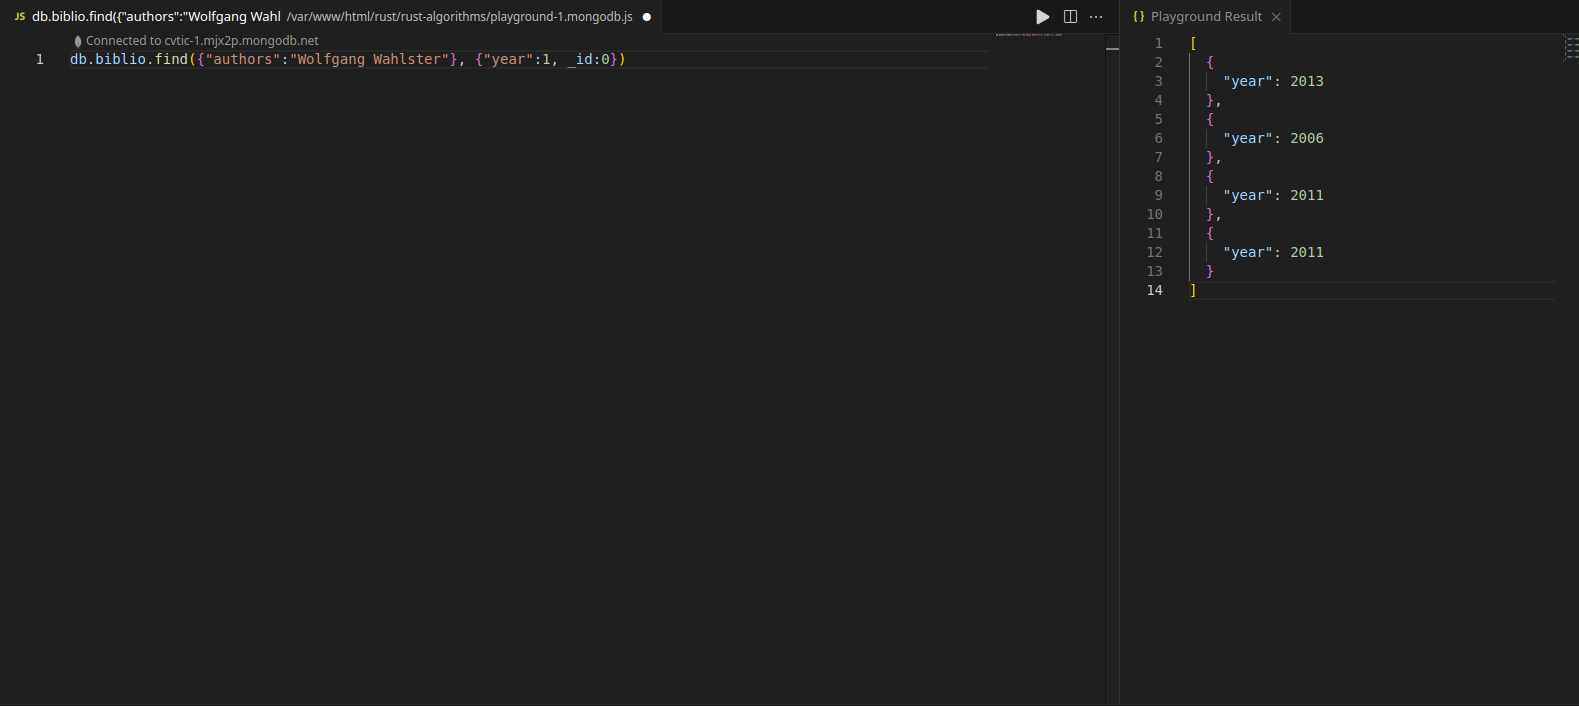
\includegraphics[scale=.4]{exos/exo_3_q_7}
\end{center}

\subsection{Afficher la liste de tous les éditeurs (champ « publisher ») distincts}

\begin{center}
	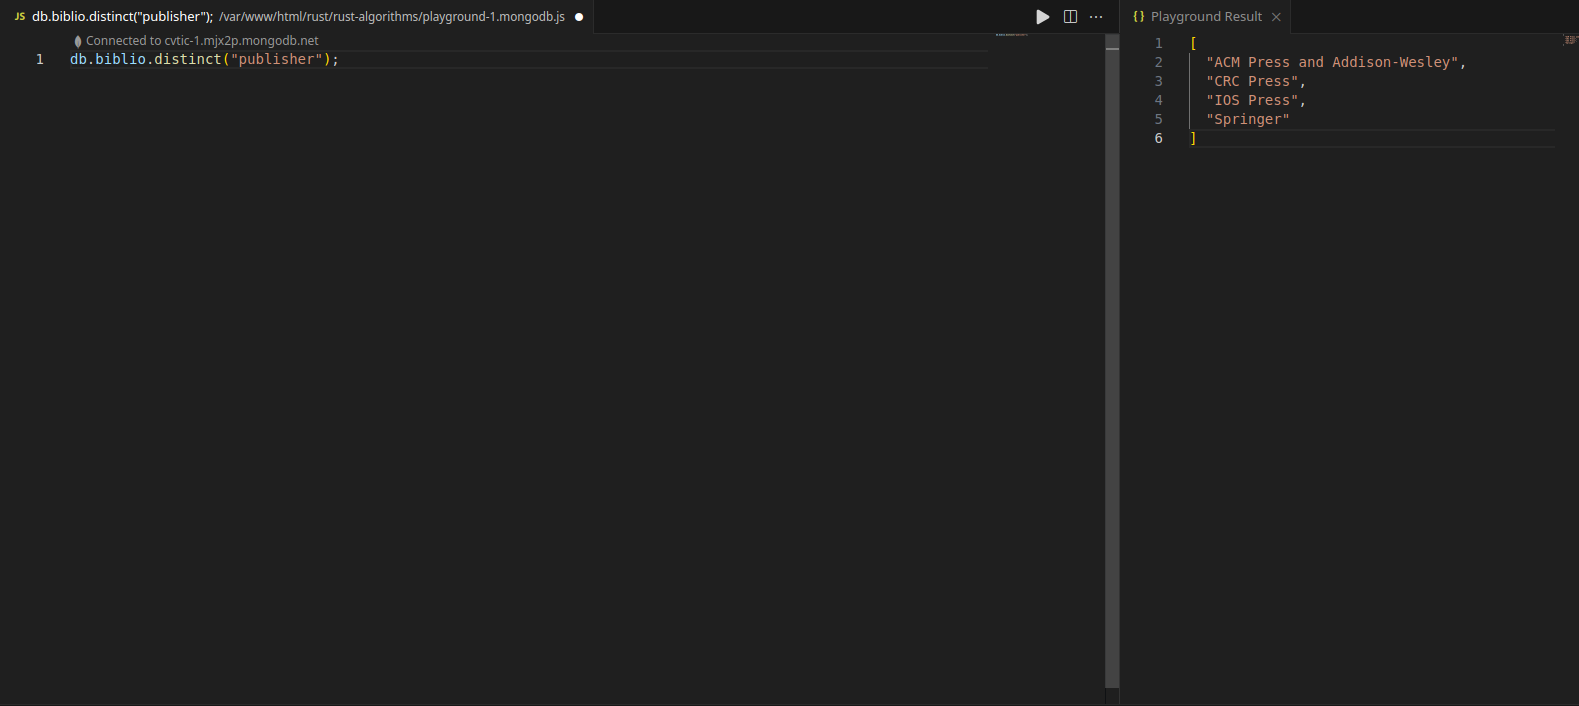
\includegraphics[scale=.4]{exos/exo_3_q_8}
\end{center}

\subsection{Afficher la liste des publications de « Wolfgang Wahlster » triée par année croissante}

\begin{center}
	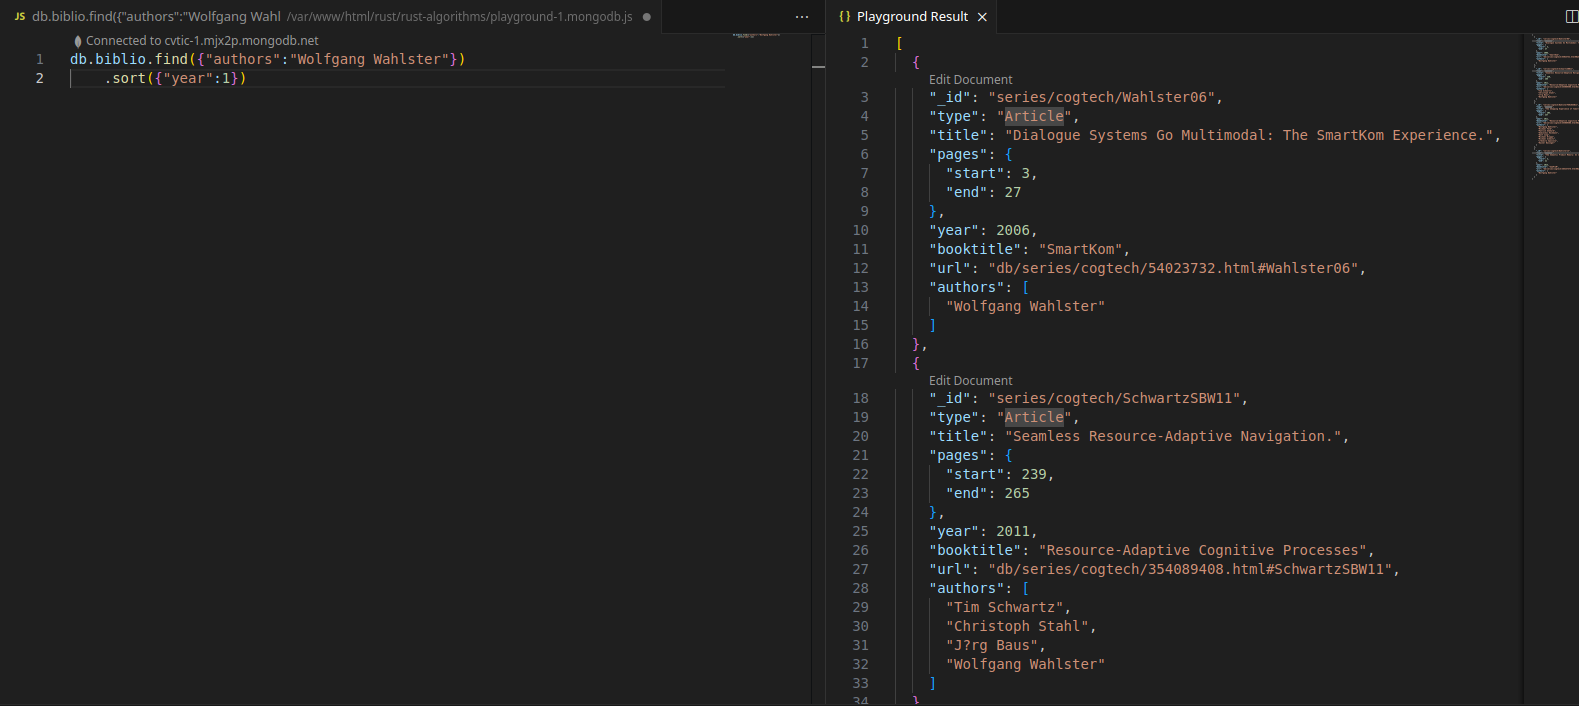
\includegraphics[scale=.4]{exos/exo_3_q_9}
\end{center}

\subsection{Supprimer le champ « type » de toutes les publications}

\begin{center}
	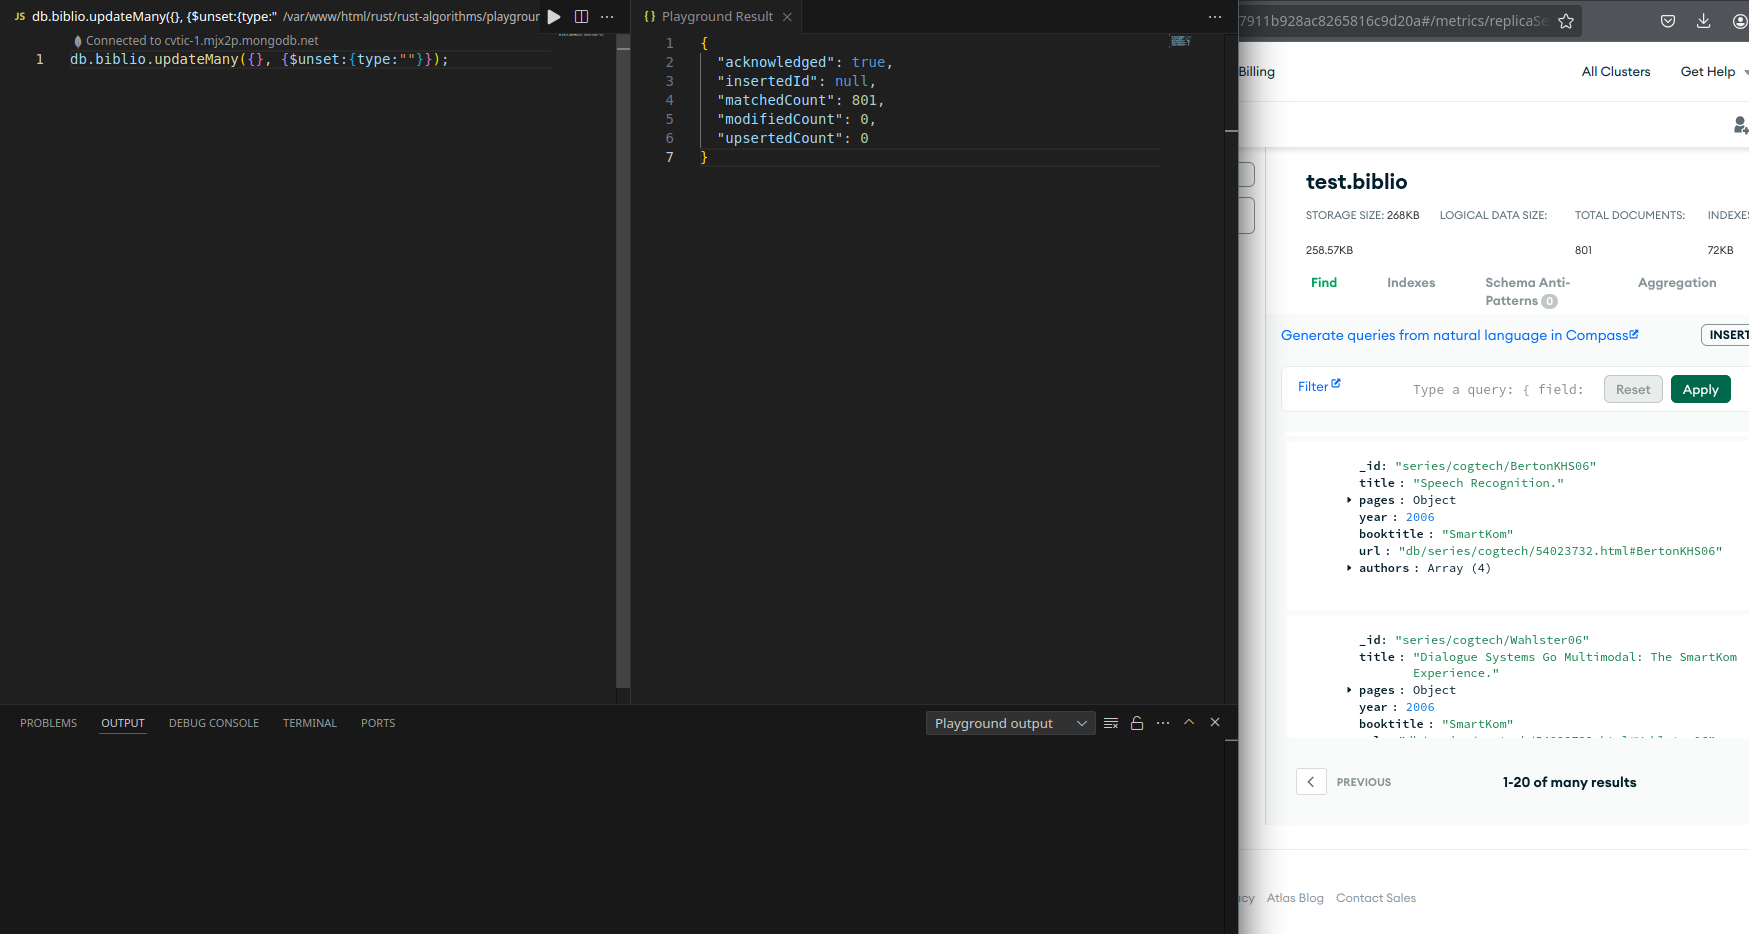
\includegraphics[scale=.35]{exos/exo_3_q_10}
\end{center}



\end{document}